%%____________________________________________________________________________||
\section{QCD multijet background estimation \label{app:qcd}}
\label{app:qcd}

\begin{figure}[!h]
  \centering
  \subfigure[Data counts.]{
    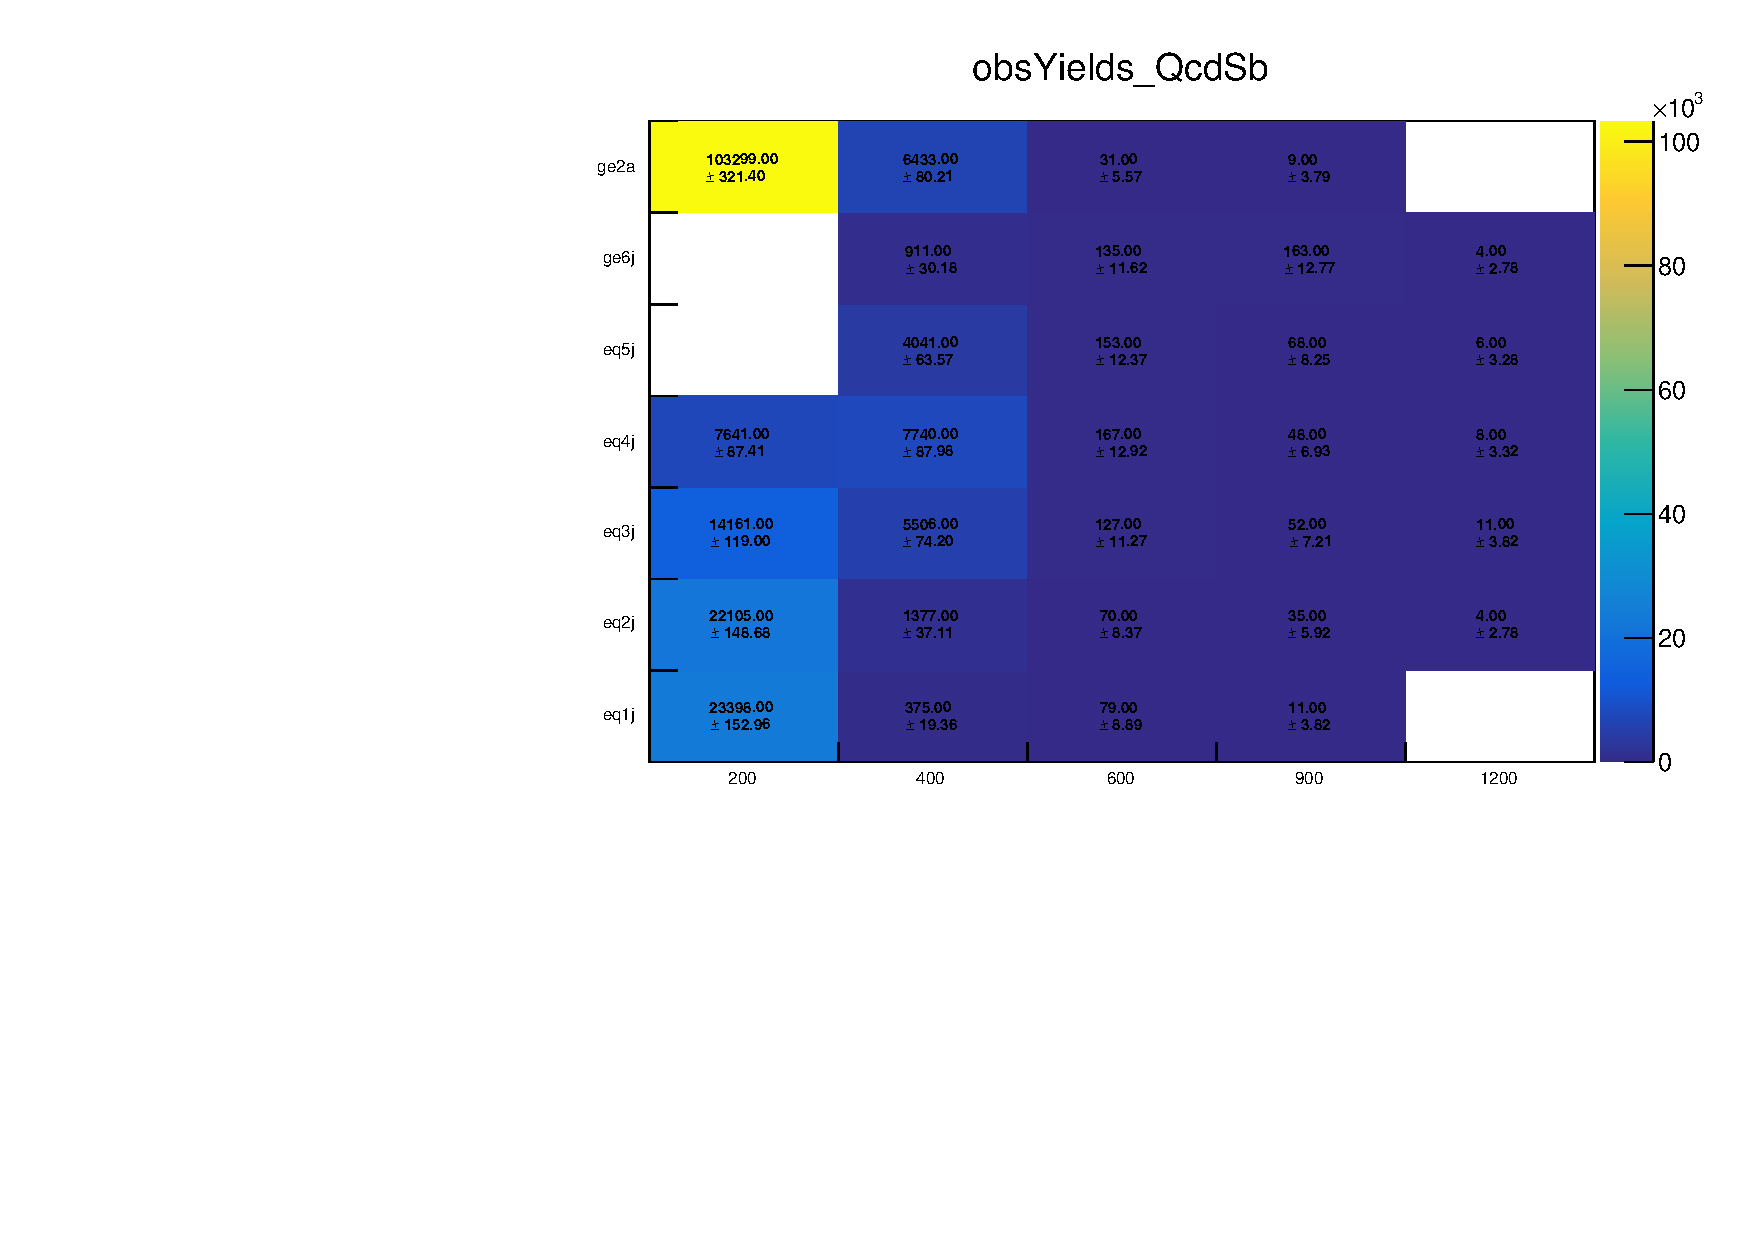
\includegraphics[width=0.5\textwidth]{figures/qcd/qcdANPlots/obsYields_QcdSb}
  } 
  \subfigure[Post-fit EWK background estimates.]{
    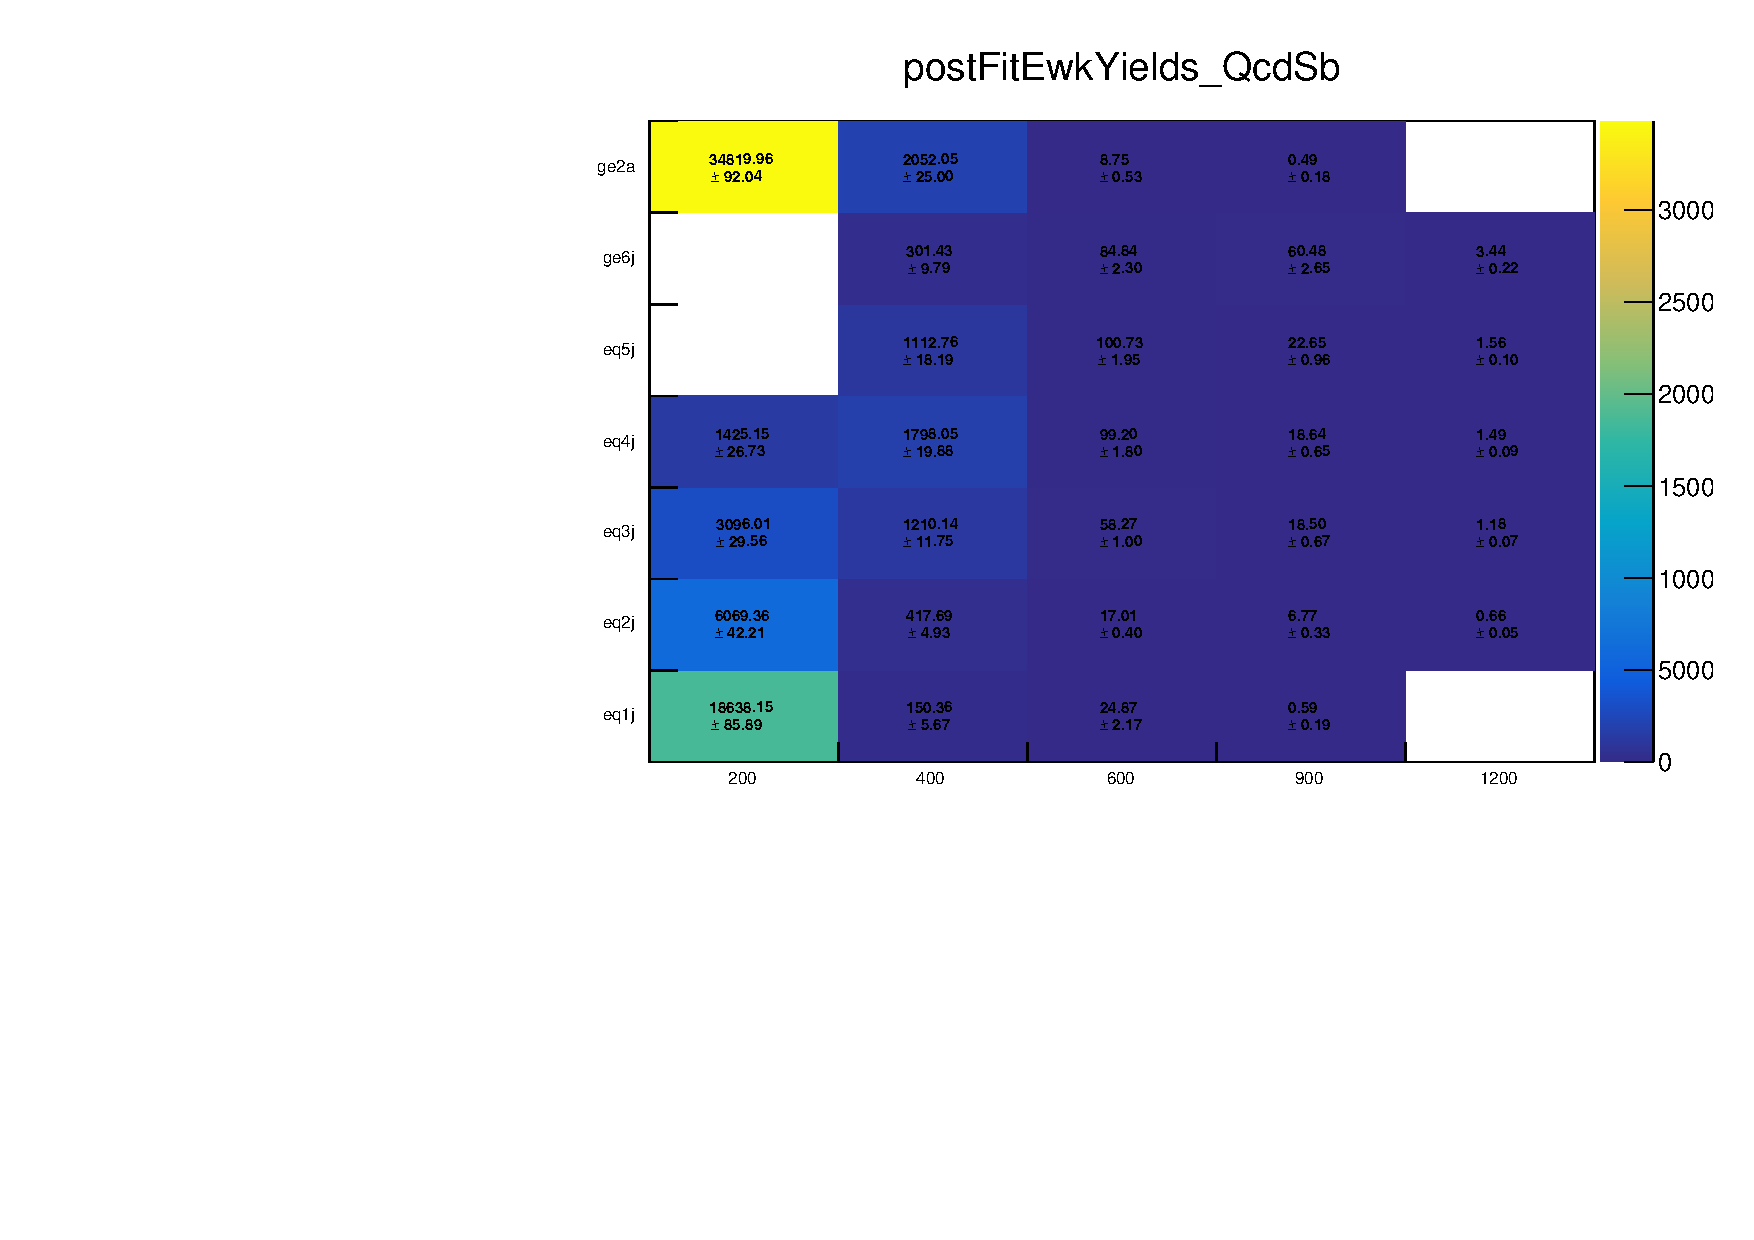
\includegraphics[width=0.5\textwidth]{figures/qcd/qcdANPlots/postFitEwkYields_QcdSb}
  } \\
  \subfigure[Post-fit QCD background estimates.]{
    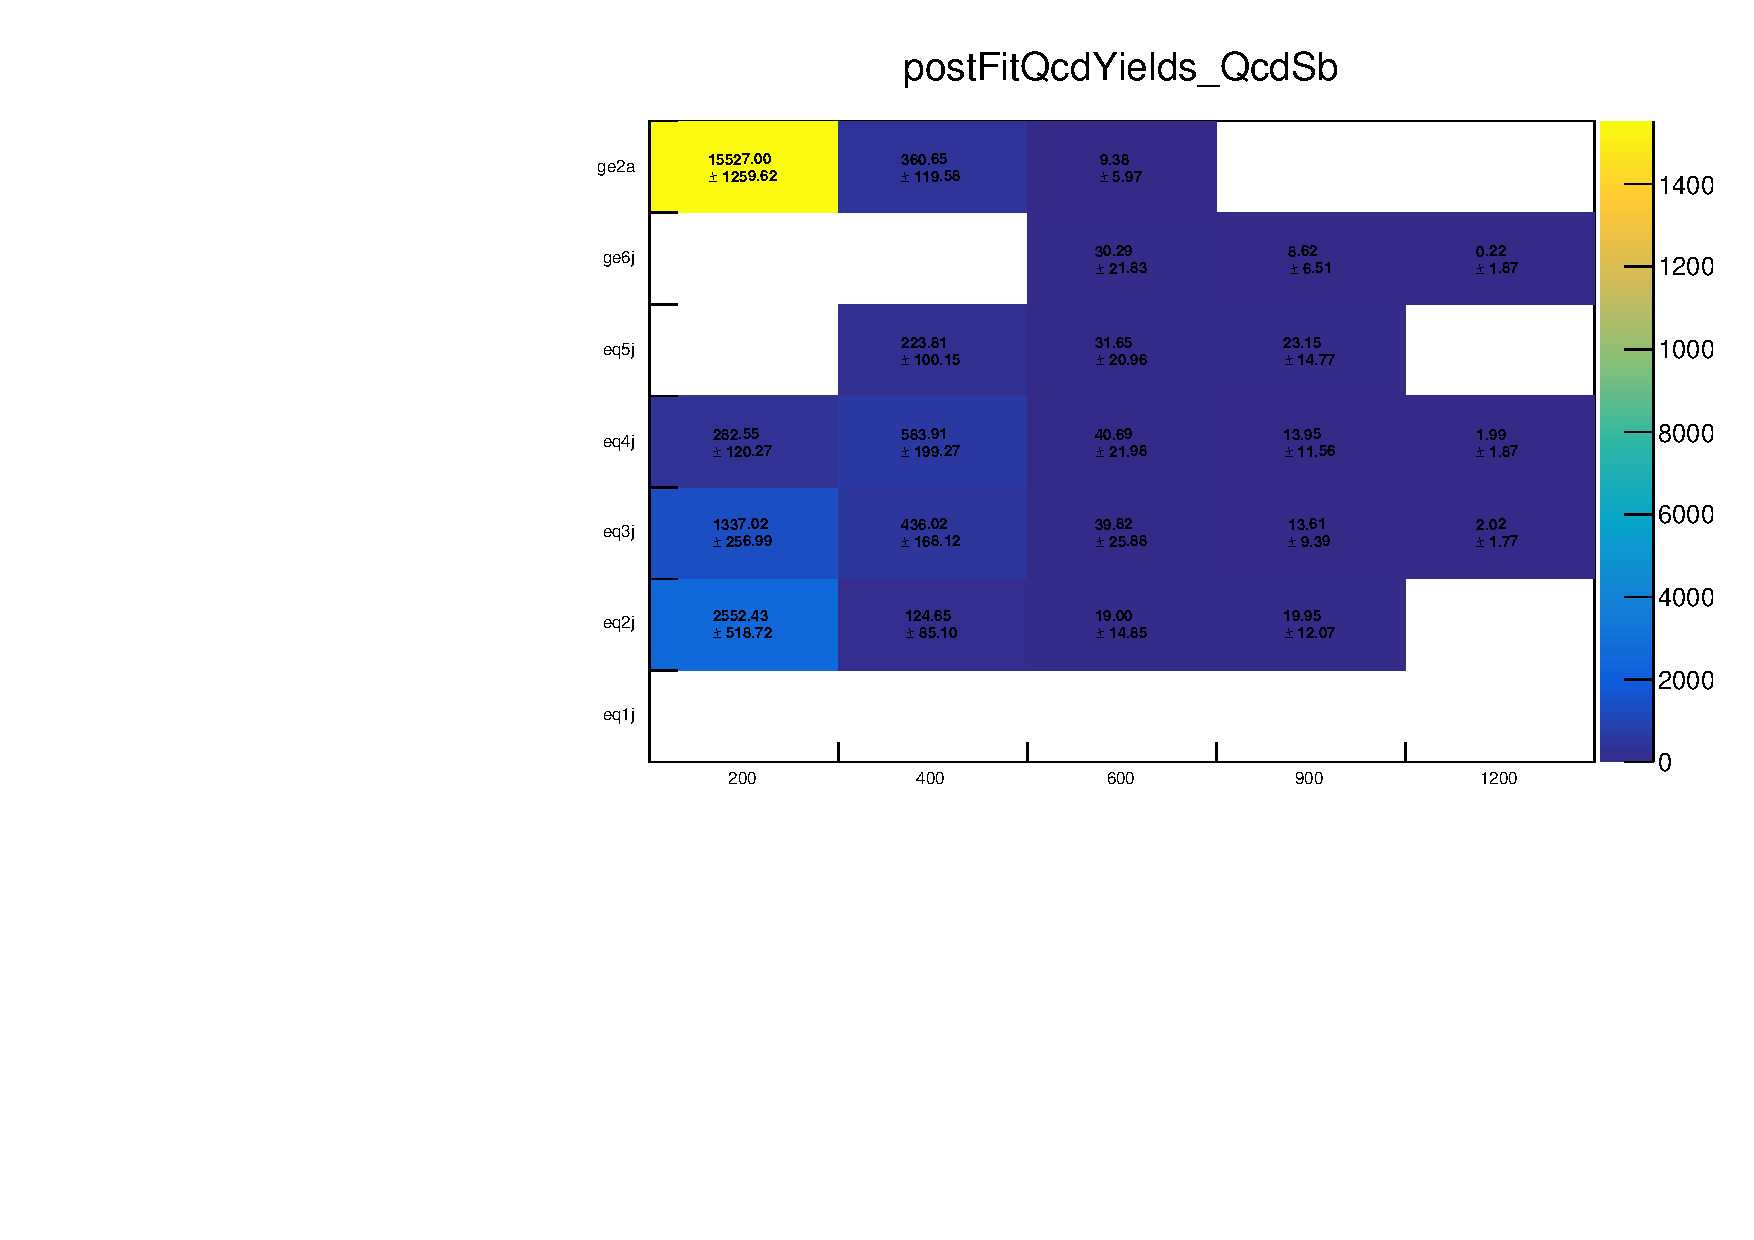
\includegraphics[width=0.5\textwidth]{figures/qcd/qcdANPlots/postFitQcdYields_QcdSb}
  } 
  \subfigure[Post-fit ML values of $\mu_{\textrm{QCD}}$.]{
    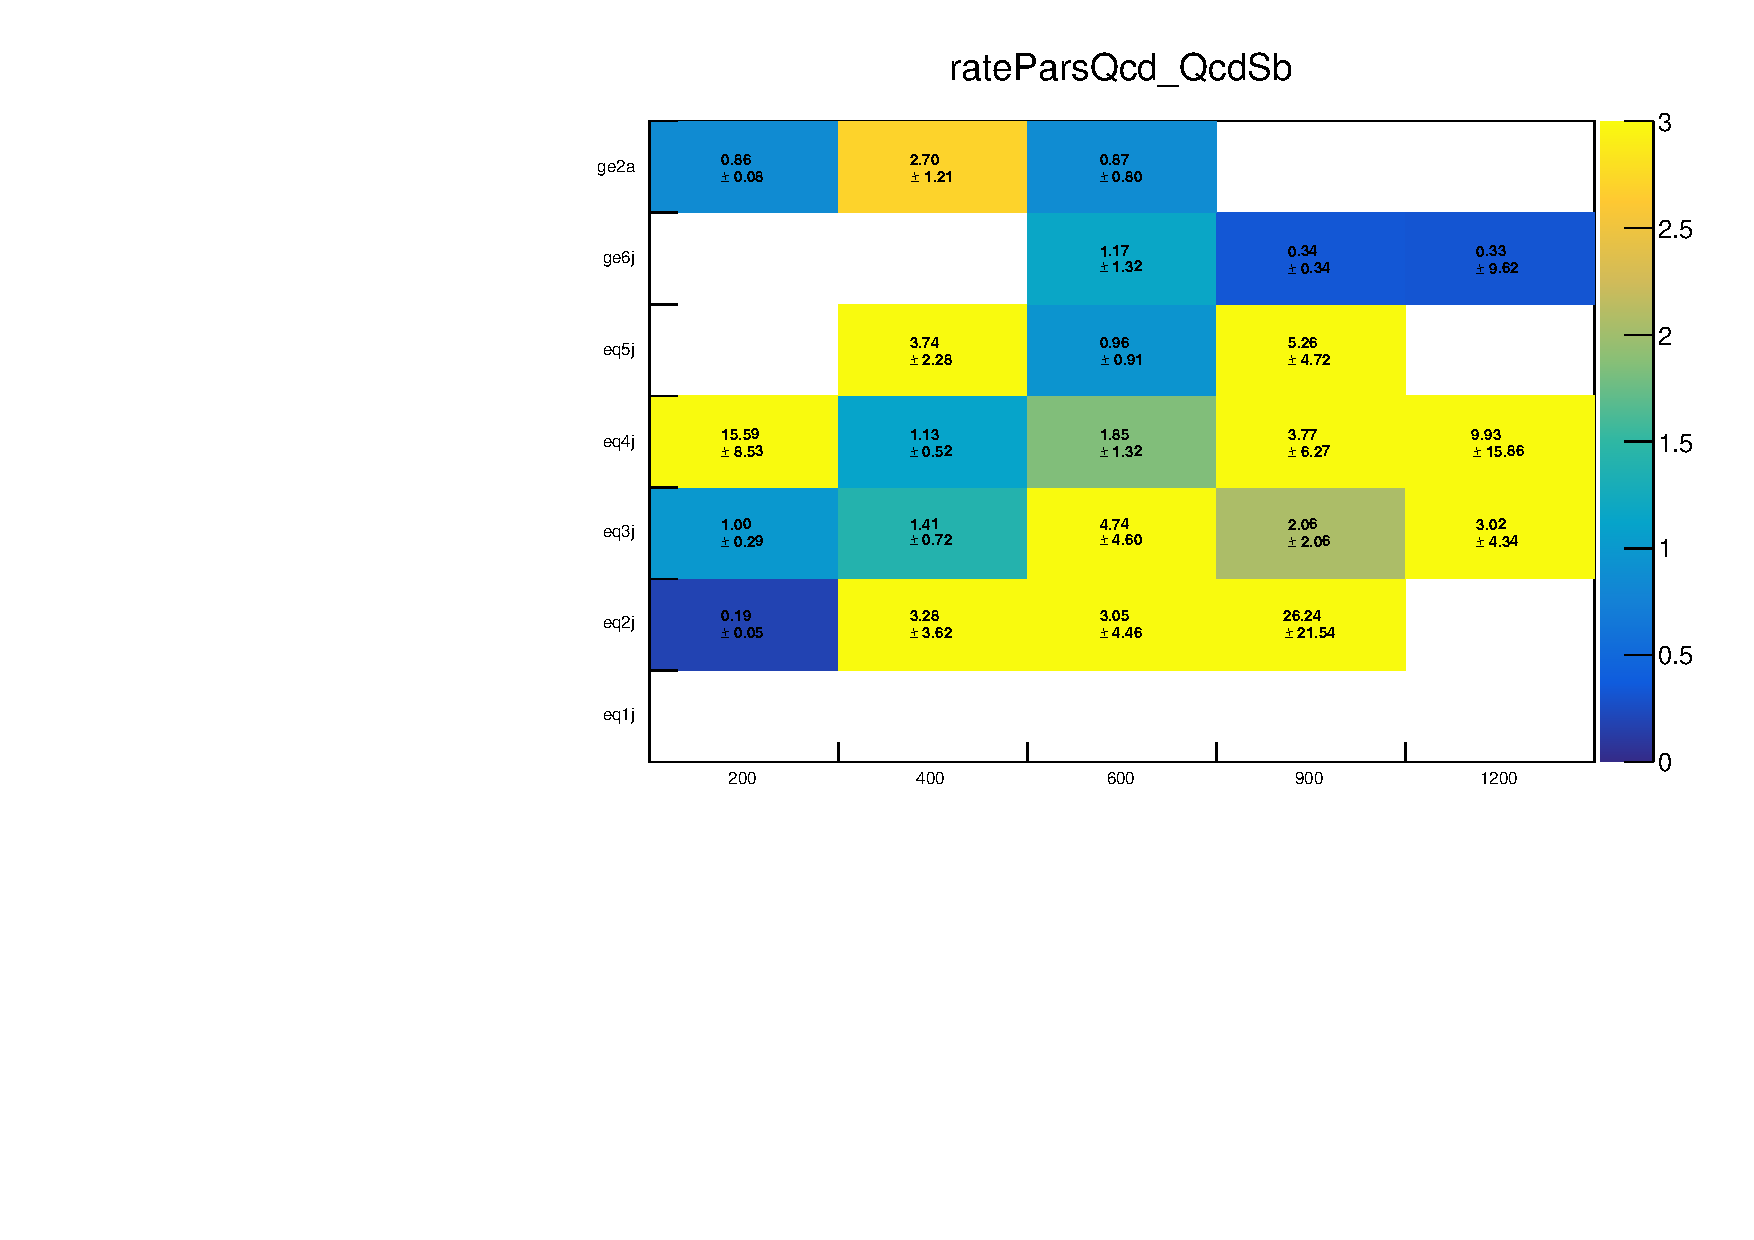
\includegraphics[width=0.5\textwidth]{figures/qcd/qcdANPlots/rateParsQcd_QcdSb}
  } \\
  \caption{Summary of the fit result in sideband \textbf{B} ($1.25 <
    \mhtmet < 3.0$) per (\njet, \scalht) bin: (a) observed data
    counts, post-fit estimates of the contributions from the (b) EWK
    and (c) QCD processes, and (d) post-fit maximum likelihood values
    of the free parameters $\mu_{\textrm{QCD}}$.}
  \label{fig:mhtmet_sideband}
\end{figure}

\clearpage
\begin{figure}[!h]
  \centering
  \subfigure[Data counts.]{
    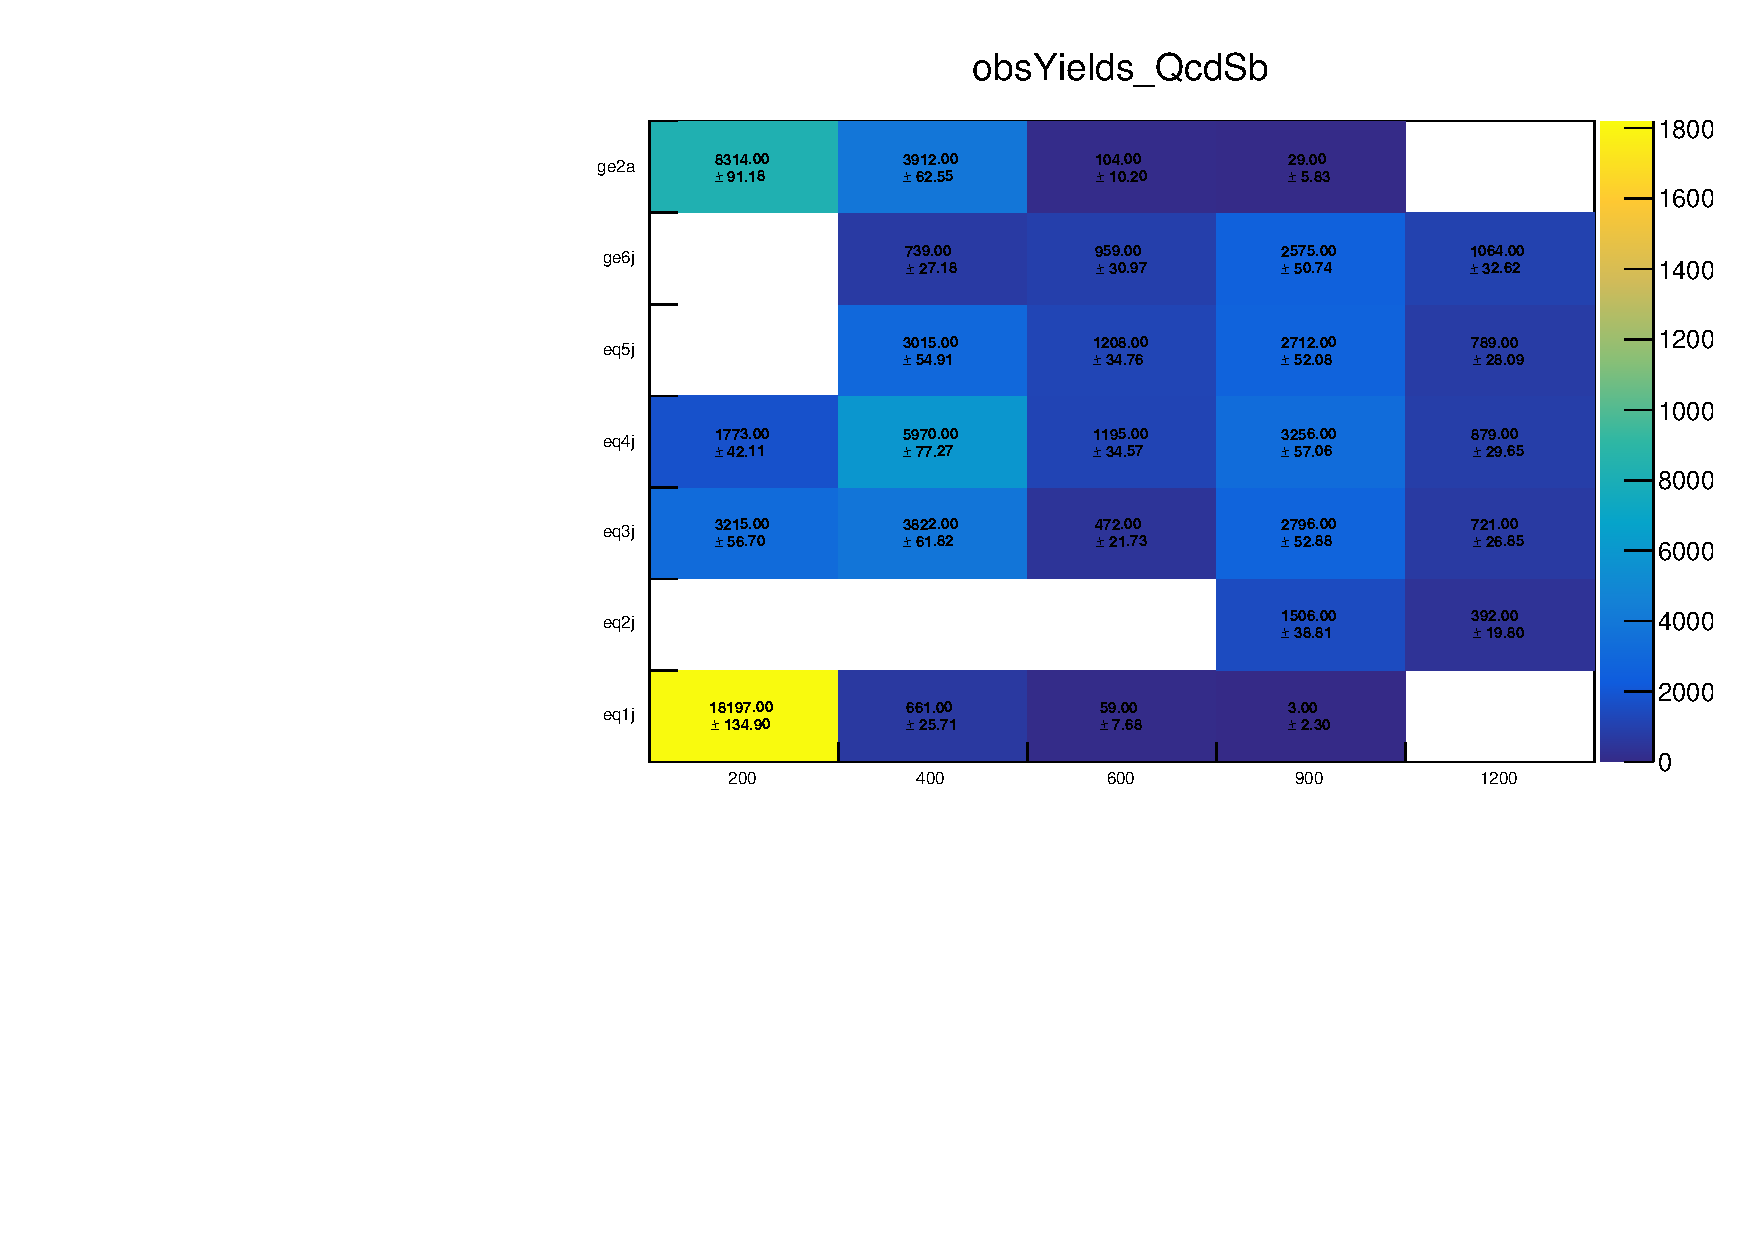
\includegraphics[width=0.5\textwidth]{figures/qcd/qcdANPlotsBDPhiSb/obsYields_QcdSb}
  } 
  \subfigure[Post-fit EWK background estimates.]{
    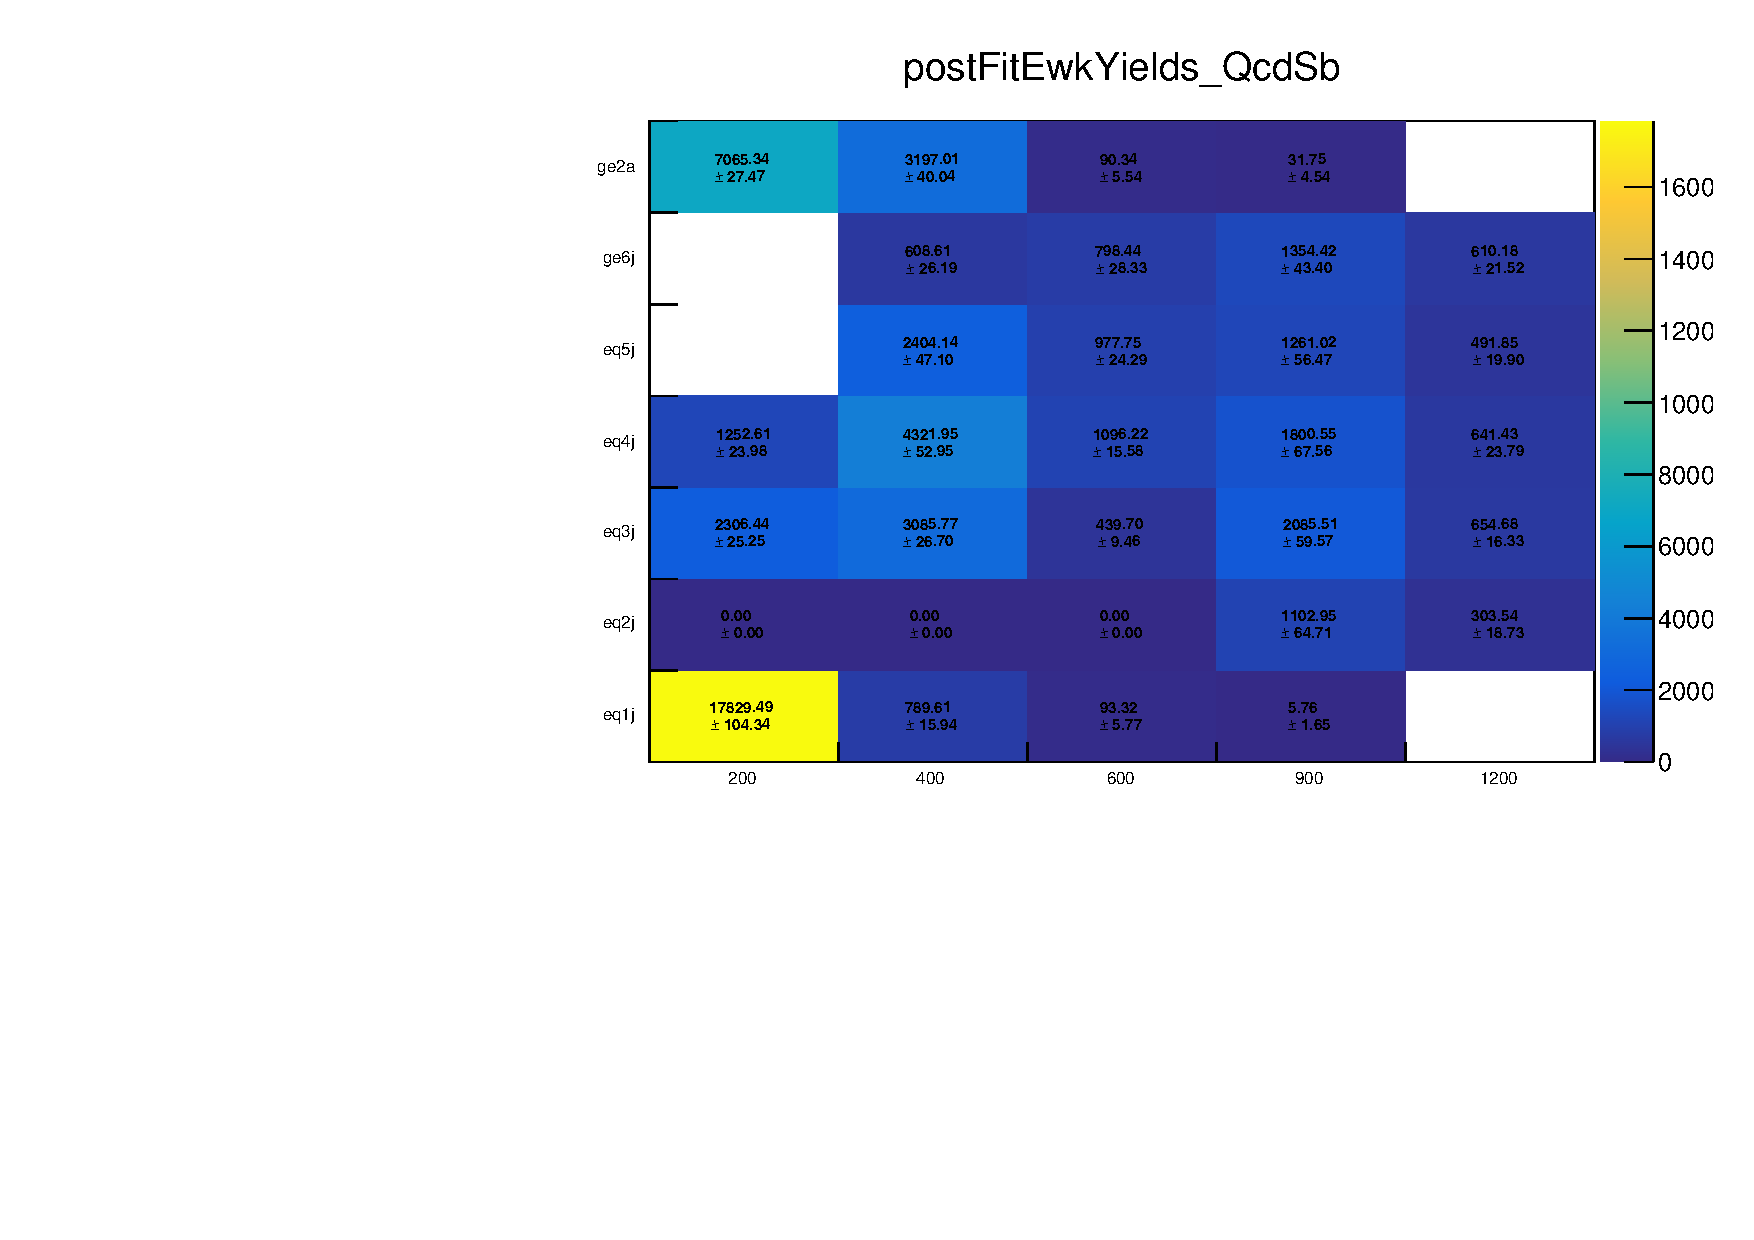
\includegraphics[width=0.5\textwidth]{figures/qcd/qcdANPlotsBDPhiSb/postFitEwkYields_QcdSb}
  } \\
  \subfigure[Post-fit QCD background estimates.]{
    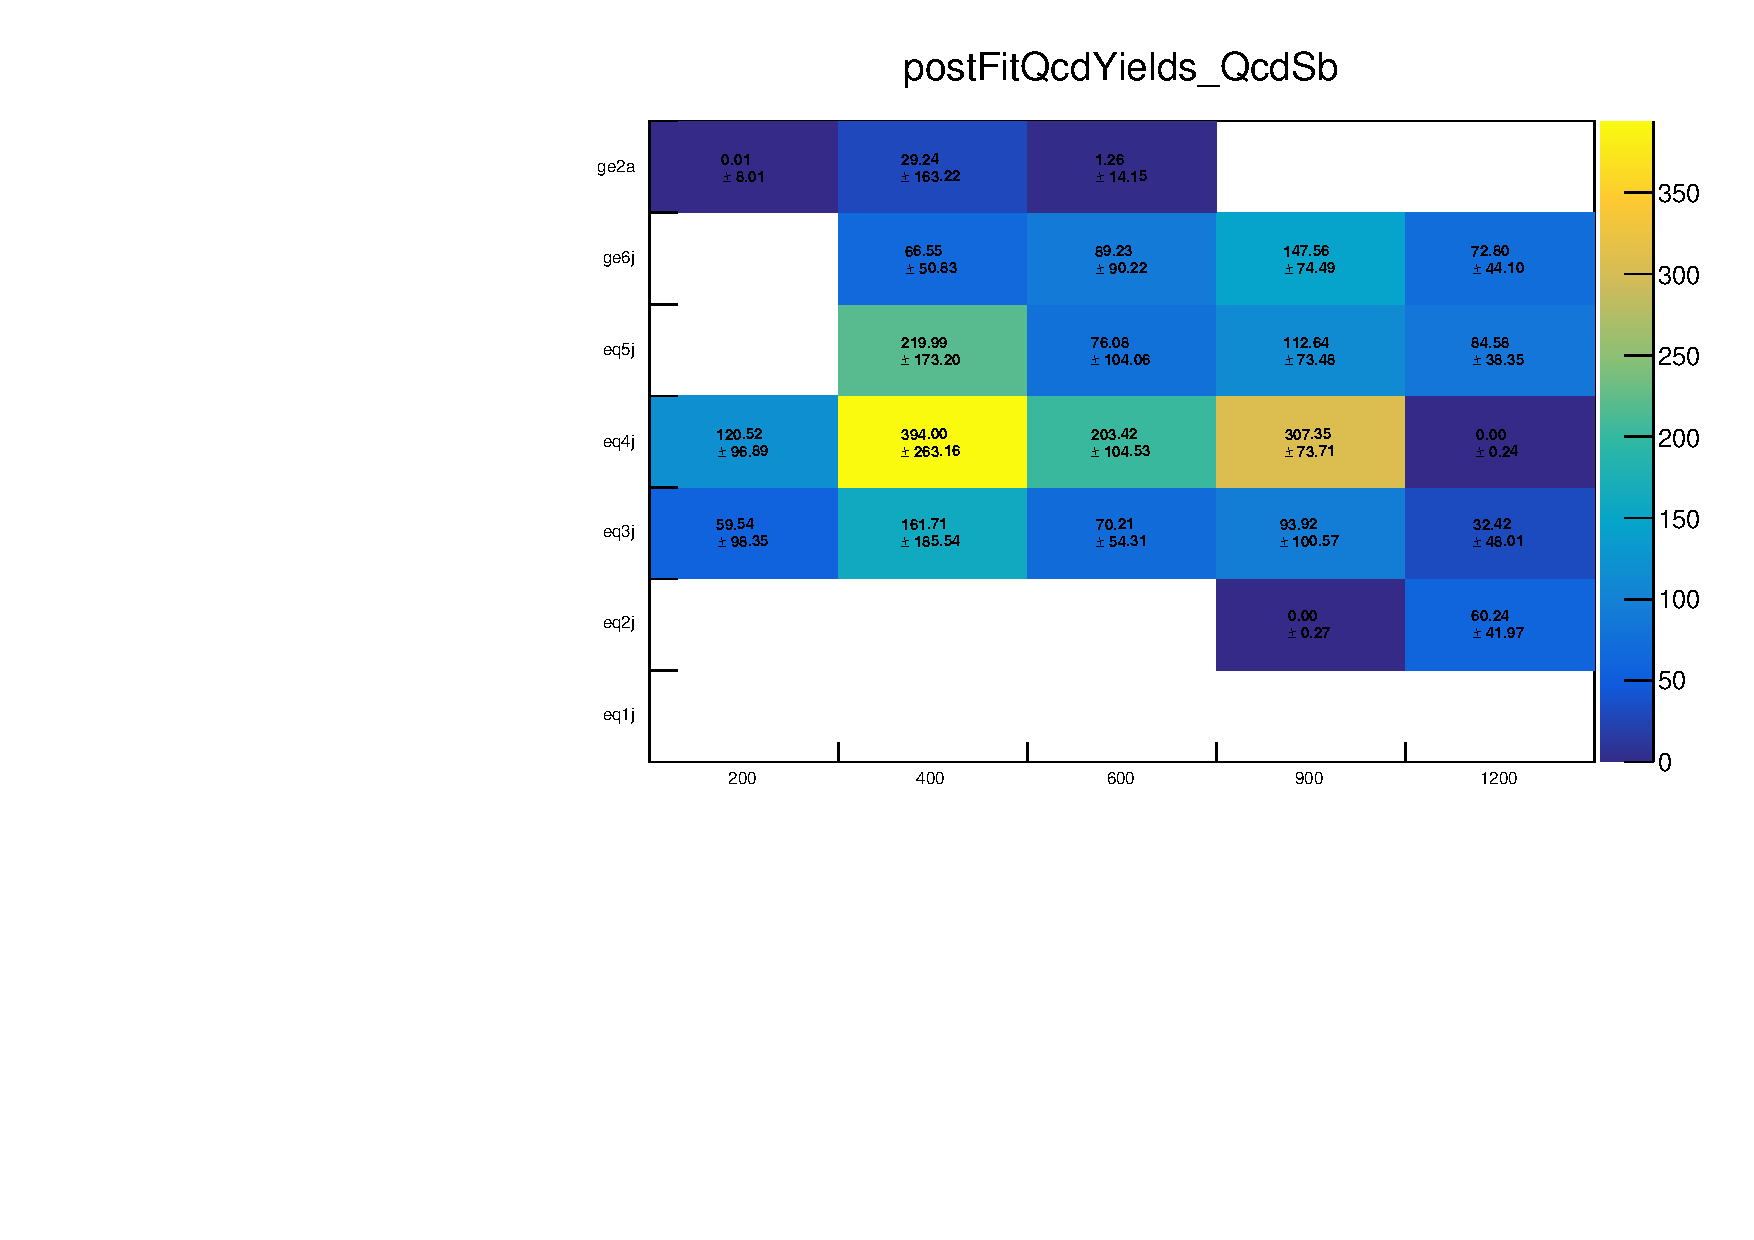
\includegraphics[width=0.5\textwidth]{figures/qcd/qcdANPlotsBDPhiSb/postFitQcdYields_QcdSb}
  } 
  \subfigure[Post-fit ML values of $\mu_{\textrm{QCD}}$.]{
    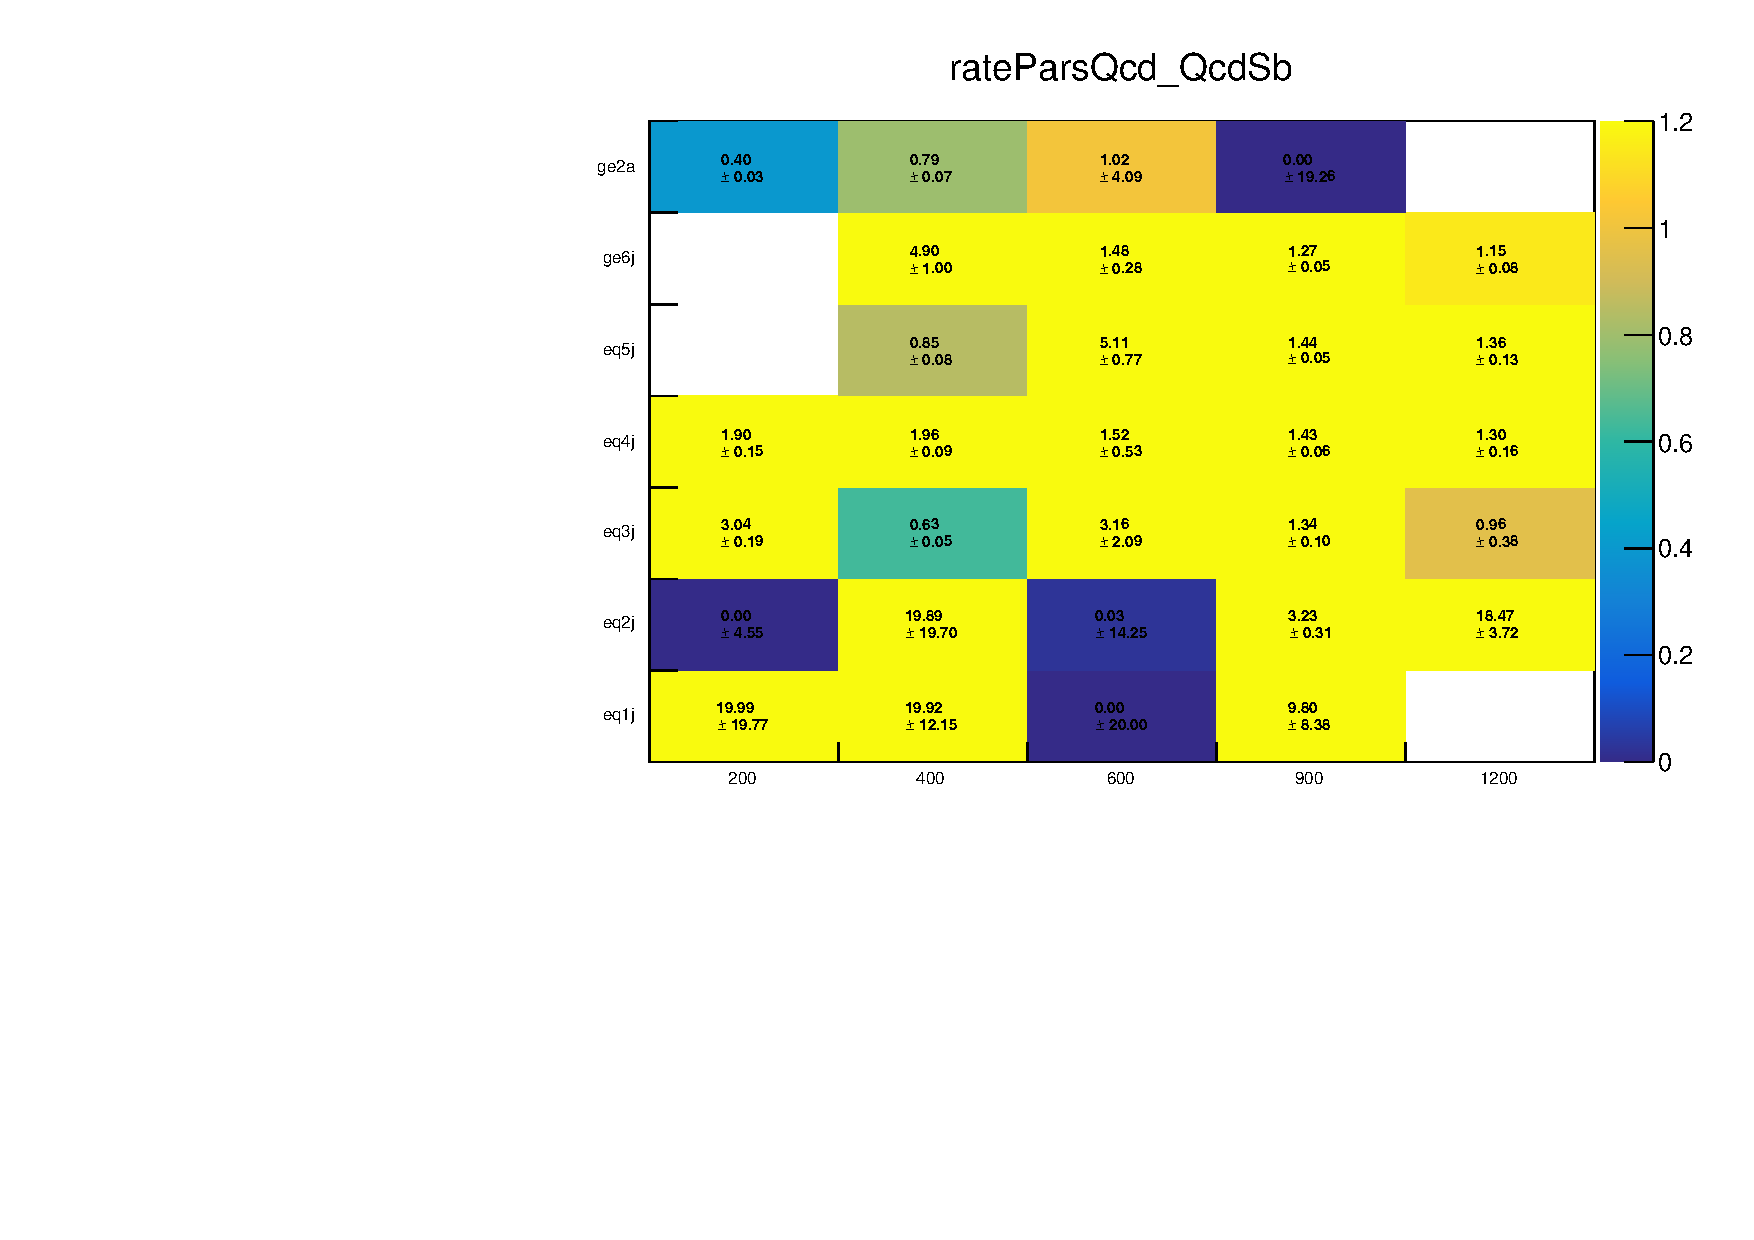
\includegraphics[width=0.5\textwidth]{figures/qcd/qcdANPlotsBDPhiSb/rateParsQcd_QcdSb}
  } \\
  \caption{Summary of the fit result in sideband \textbf{C} ($0.2 <
    \bdphi < 0.5$) per (\njet, \scalht) bin: (a) observed data counts,
    post-fit estimates of the contributions from the (b) EWK and (c)
    QCD processes, and (d) post-fit maximum likelihood values of the
    free parameters $\mu_{\textrm{QCD}}$.}
  \label{fig:bdphi_sideband}
\end{figure}

\clearpage
\begin{figure}[!h]
  \centering
  \subfigure[Data counts.]{
    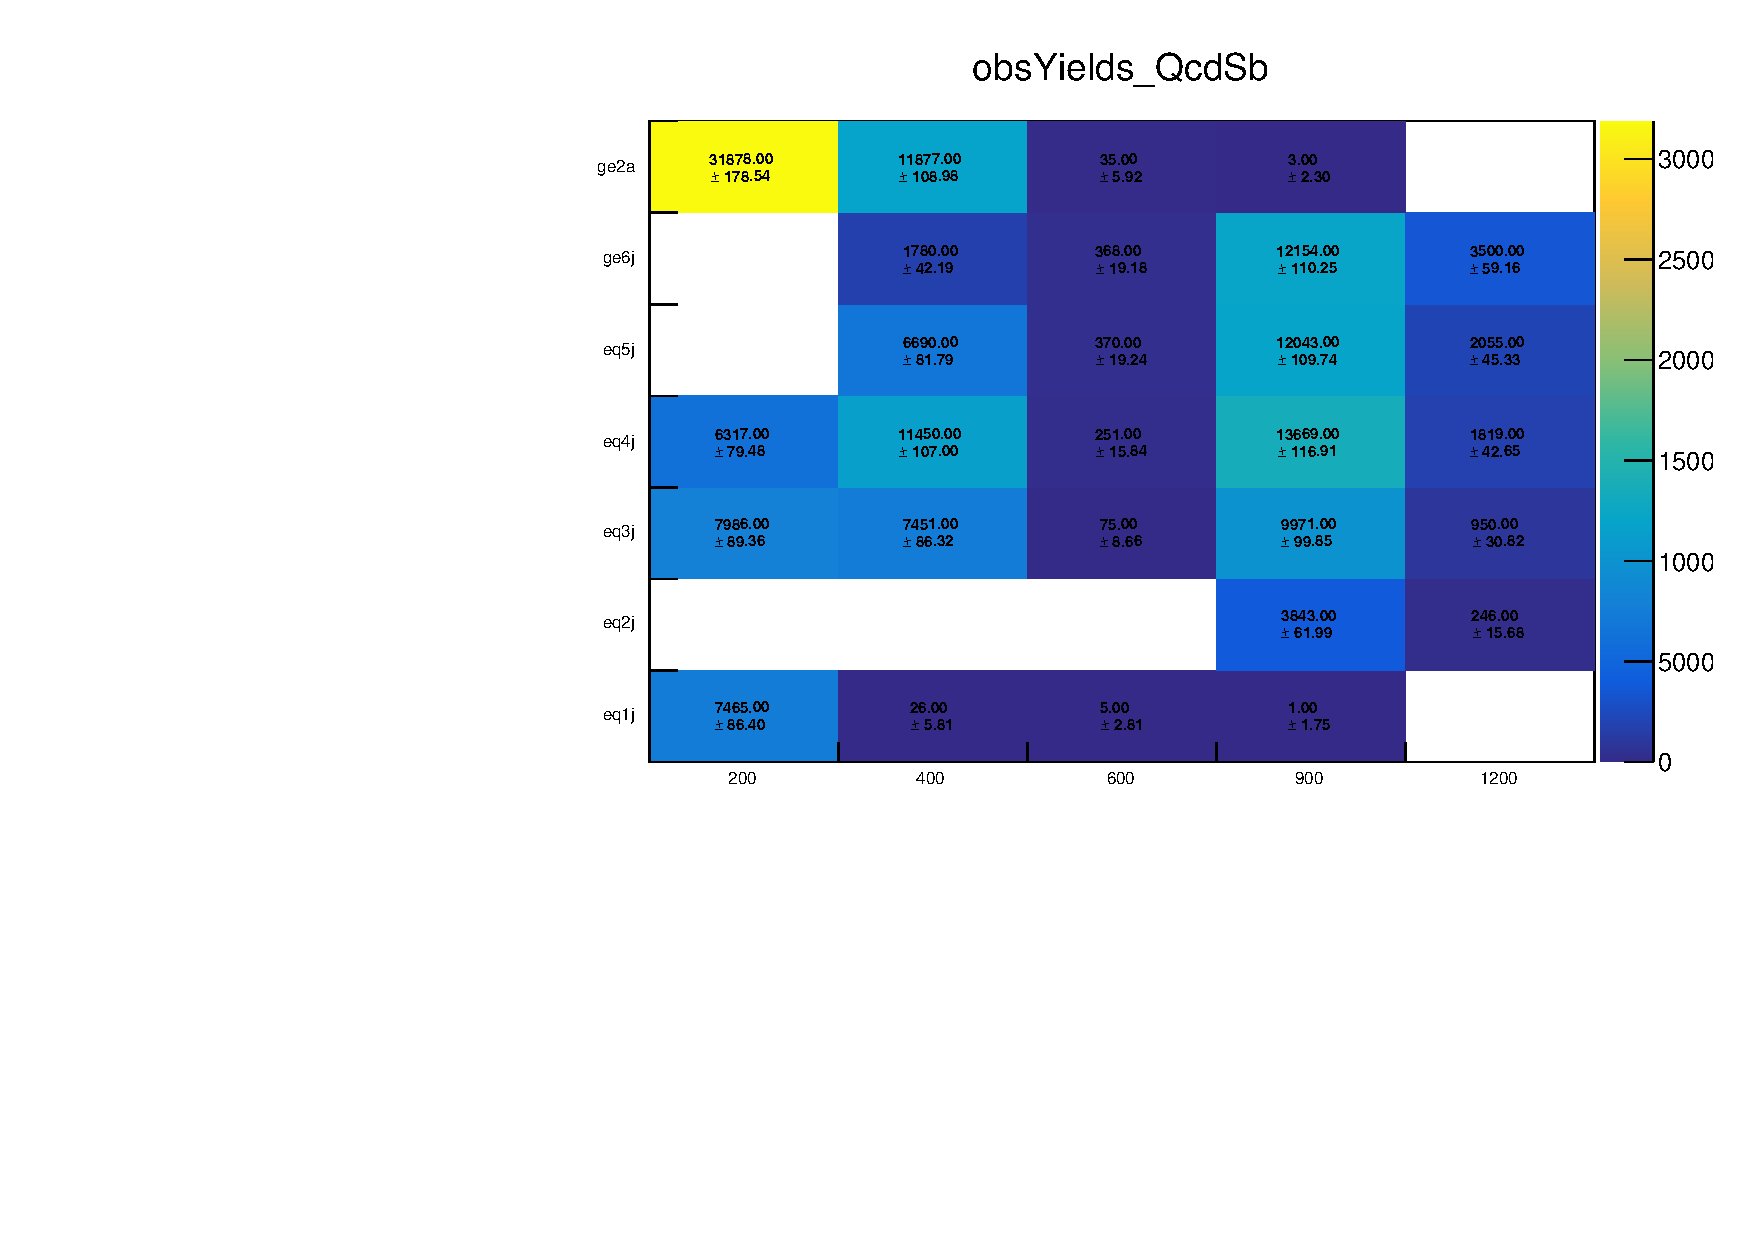
\includegraphics[width=0.5\textwidth]{figures/qcd/qcdANPlotsDoubleSb/obsYields_QcdSb}
  } 
  \subfigure[Post-fit EWK background estimates.]{
    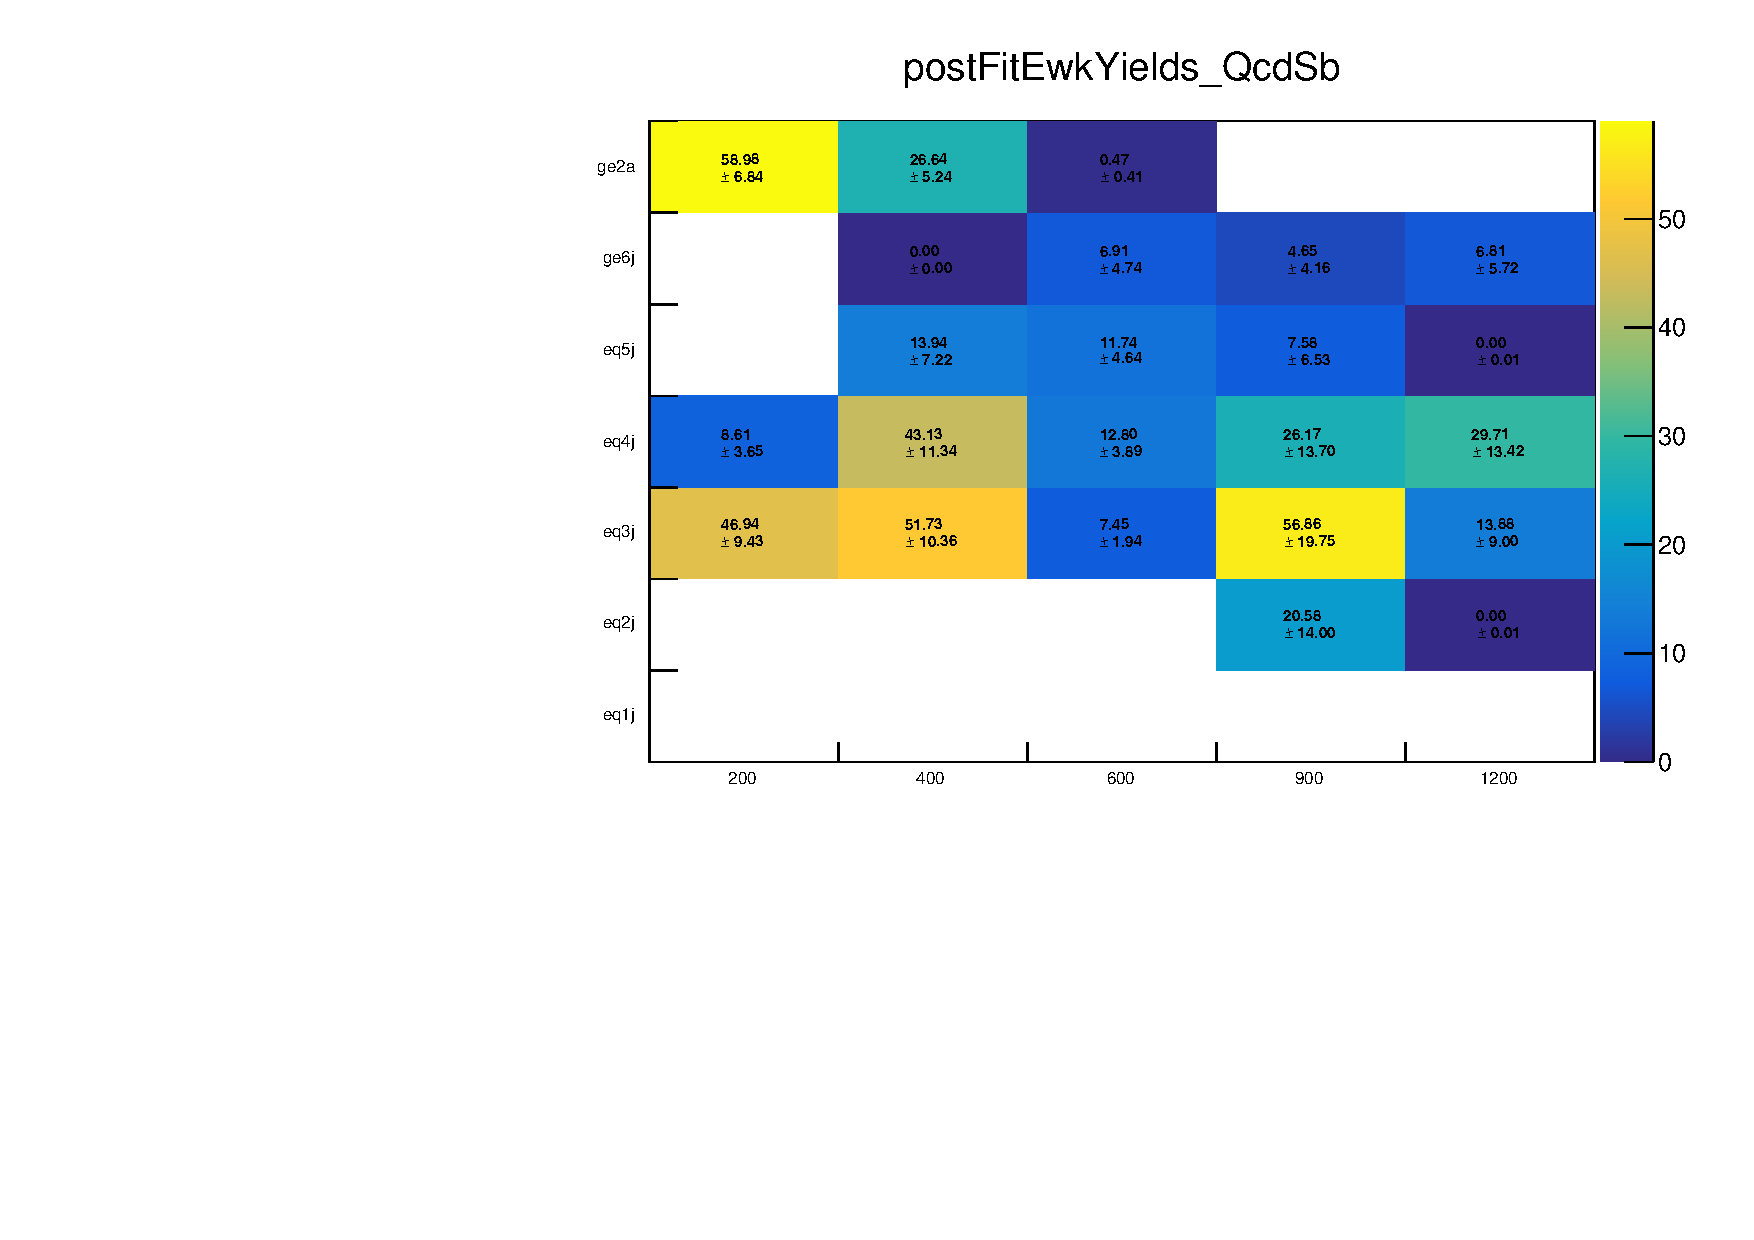
\includegraphics[width=0.5\textwidth]{figures/qcd/qcdANPlotsDoubleSb/postFitEwkYields_QcdSb}
  } \\
  \subfigure[Post-fit QCD background estimates.]{
    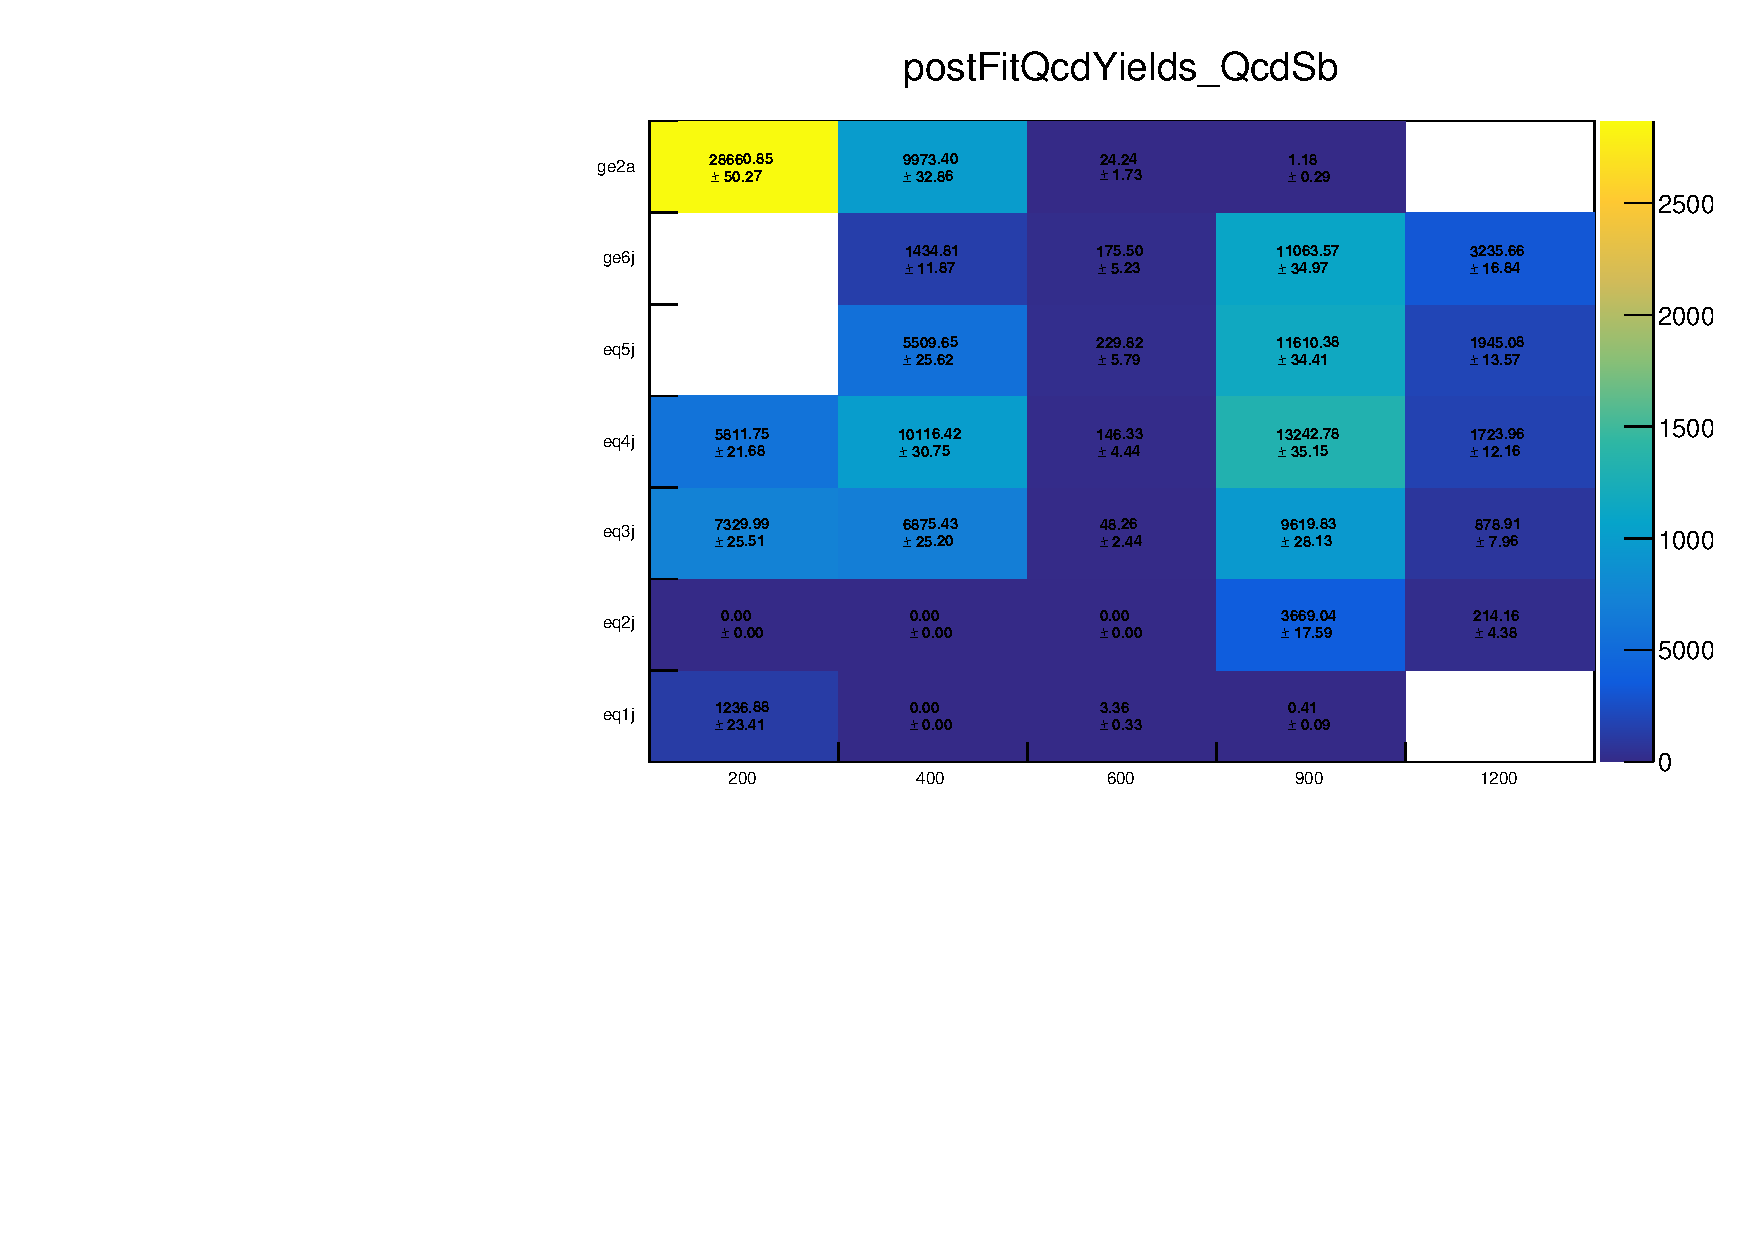
\includegraphics[width=0.5\textwidth]{figures/qcd/qcdANPlotsDoubleSb/postFitQcdYields_QcdSb}
  } 
  \subfigure[Post-fit ML values of $\mu_{\textrm{QCD}}$.]{
    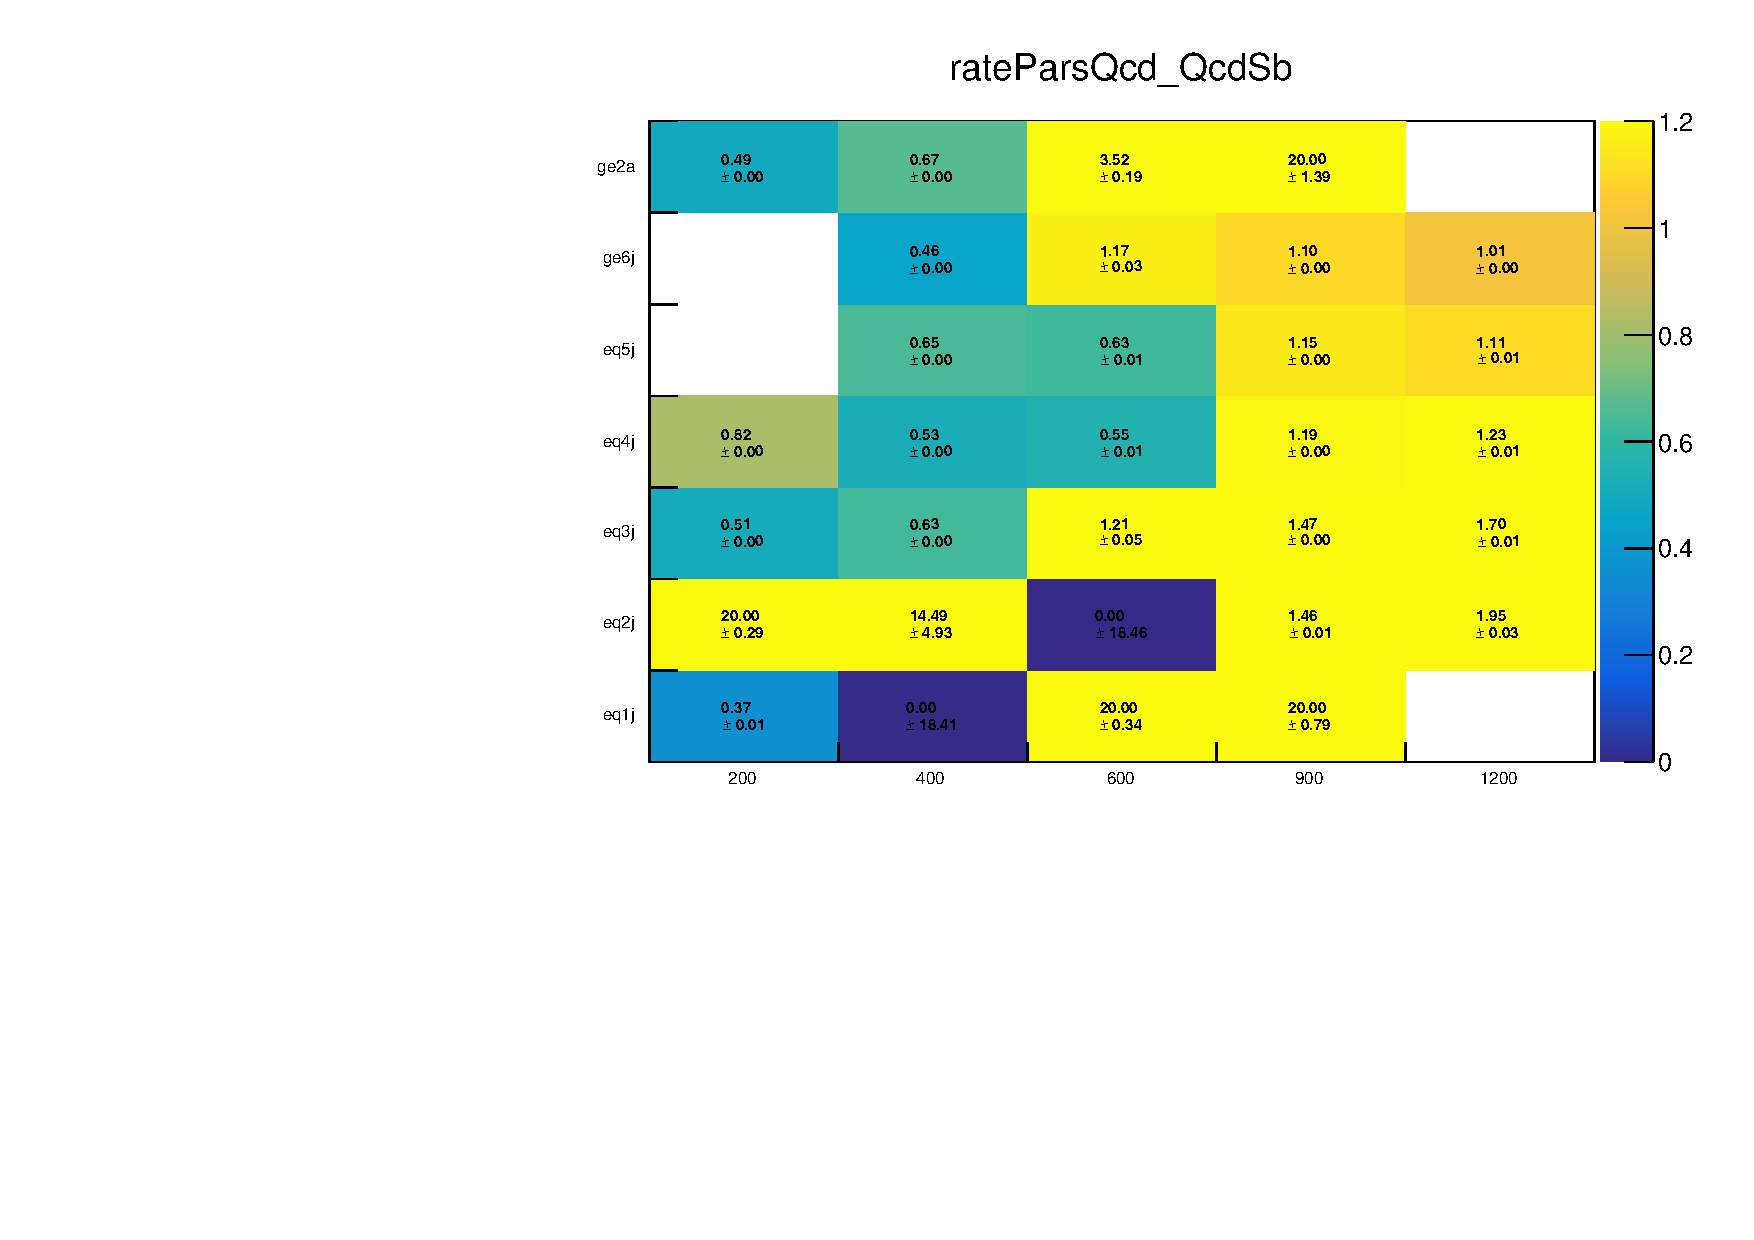
\includegraphics[width=0.5\textwidth]{figures/qcd/qcdANPlotsDoubleSb/rateParsQcd_QcdSb}
  } \\
  \caption{Summary of the fit result in the ``double'' sideband
    \textbf{A} per (\njet, \scalht) bin: (a) observed data counts,
    post-fit estimates of the contributions from the (b) EWK and (c)
    QCD processes, and (d) post-fit maximum likelihood values of the
    free parameters $\mu_{\textrm{QCD}}$.}
  \label{fig:double_sideband}
\end{figure}

\clearpage
\begin{figure}[!h]
  \centering
%  \subfigure[Pass/fail ratios \rmhtmet.]{
%    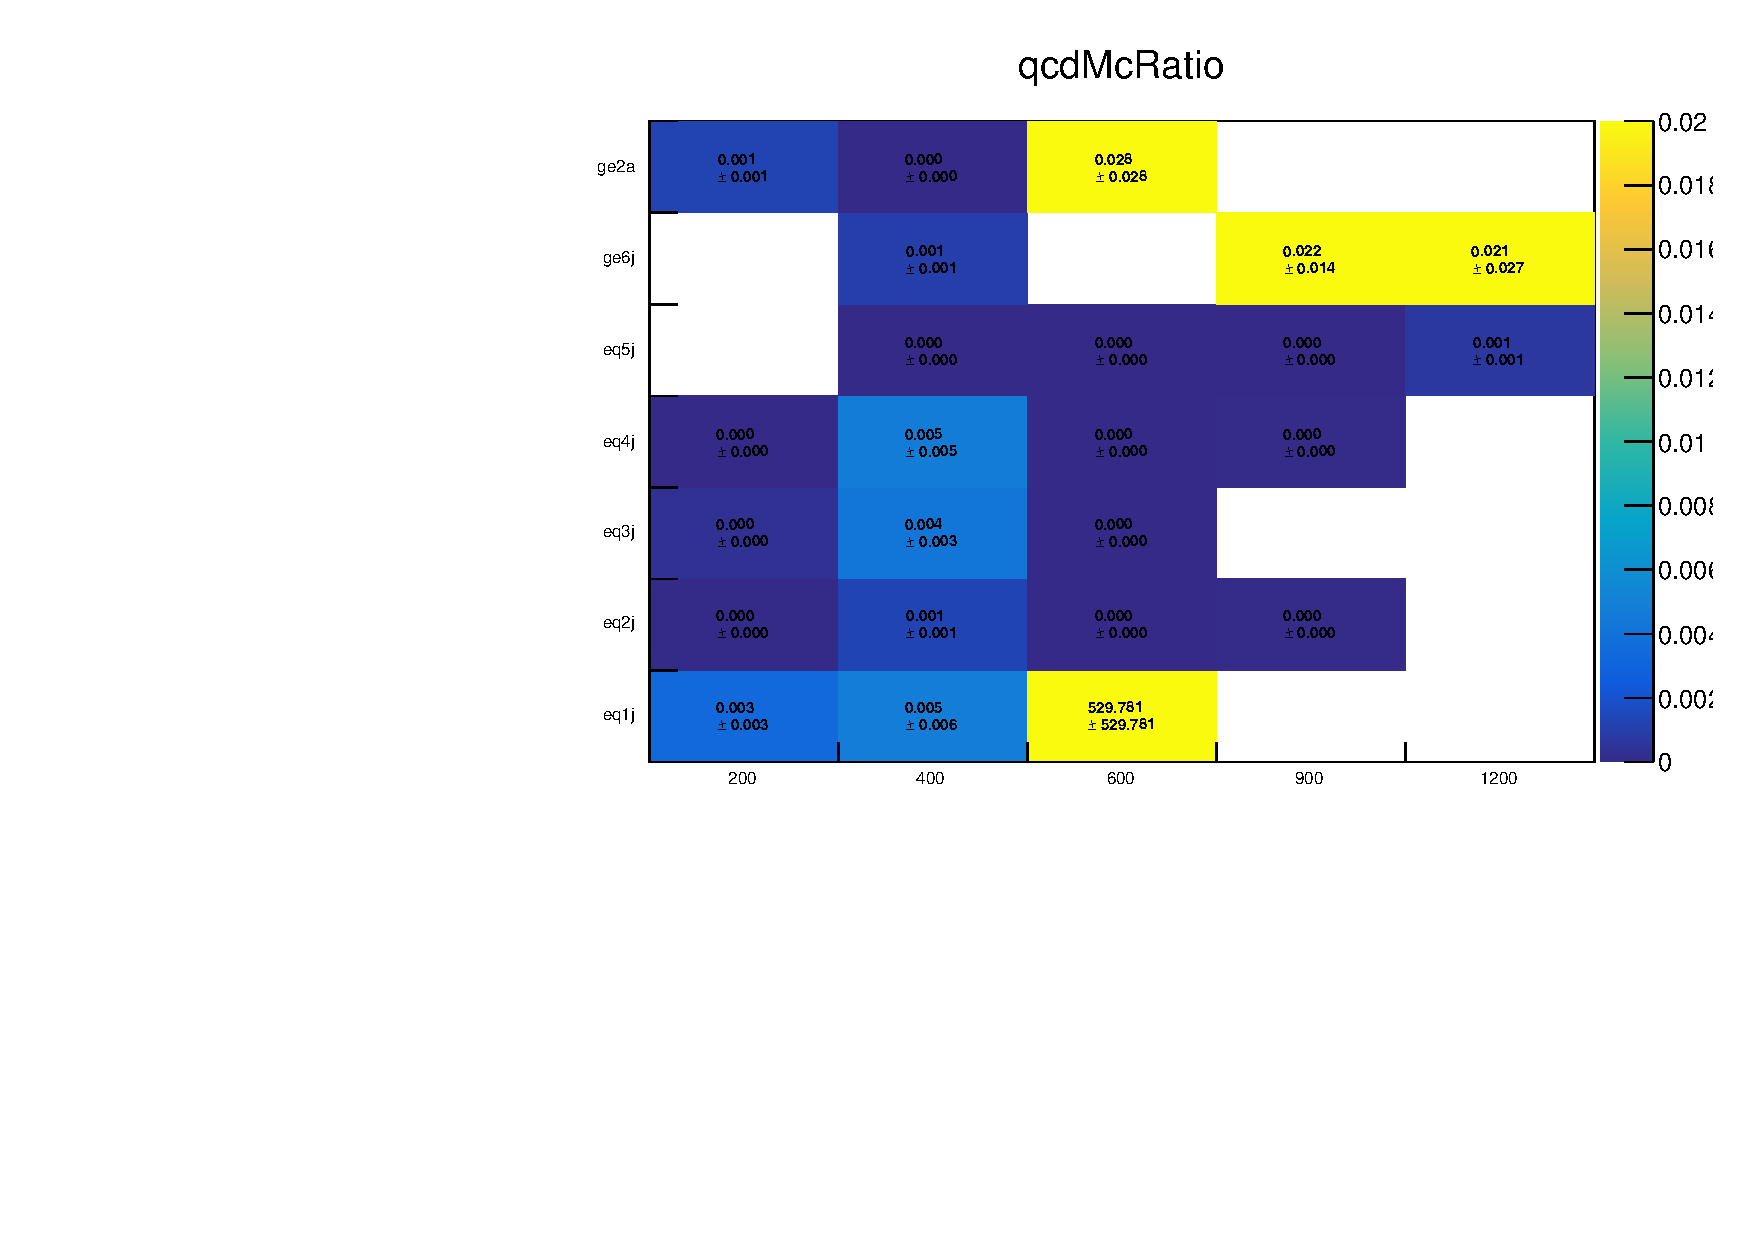
\includegraphics[width=0.5\textwidth]{figures/qcd/qcdANPlots/signalQcdDivSbQcd_MC}
%  } 
  \subfigure[QCD background estimates.]{
    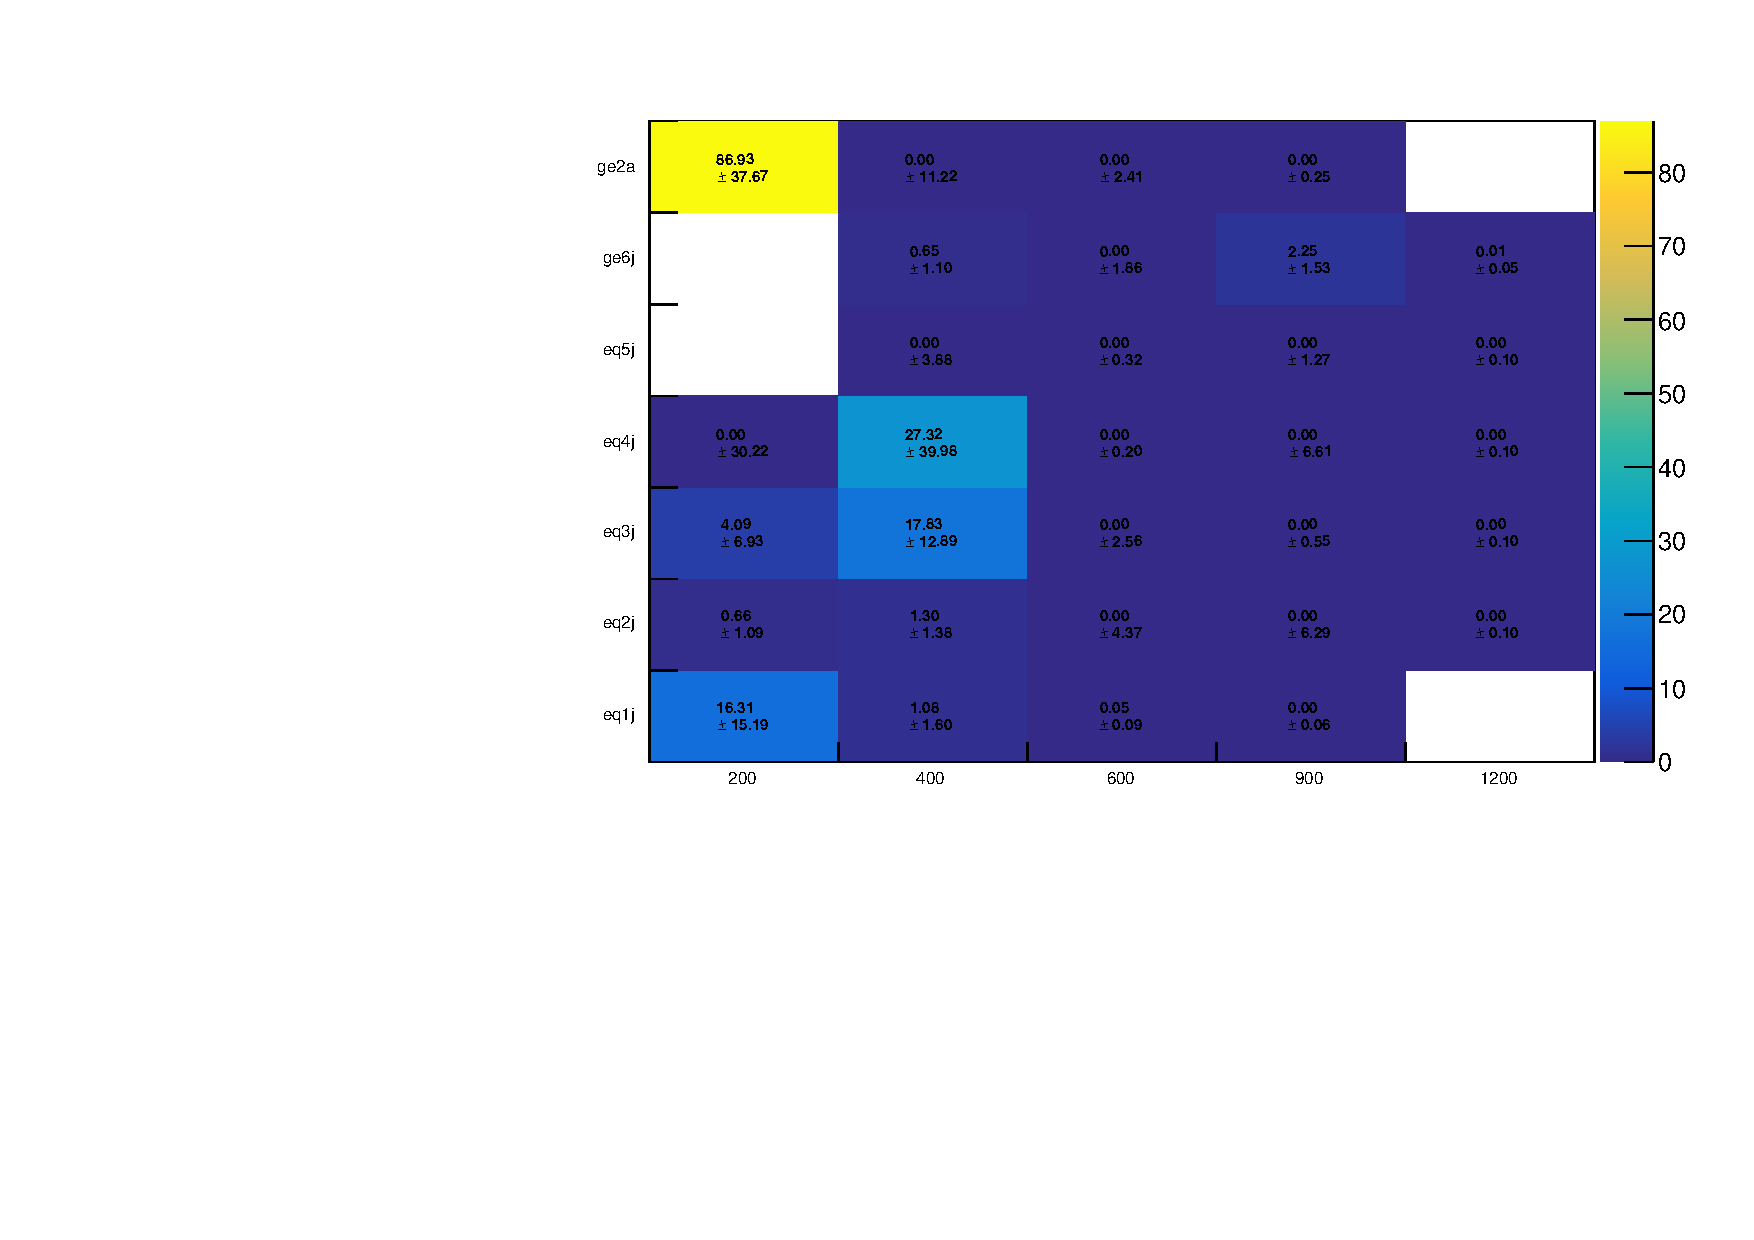
\includegraphics[width=0.6\textwidth]{figures/qcd/qcdANPlots/predictedQcdYields_Signal}
  } \\
  \subfigure[EWK background estimates.]{
    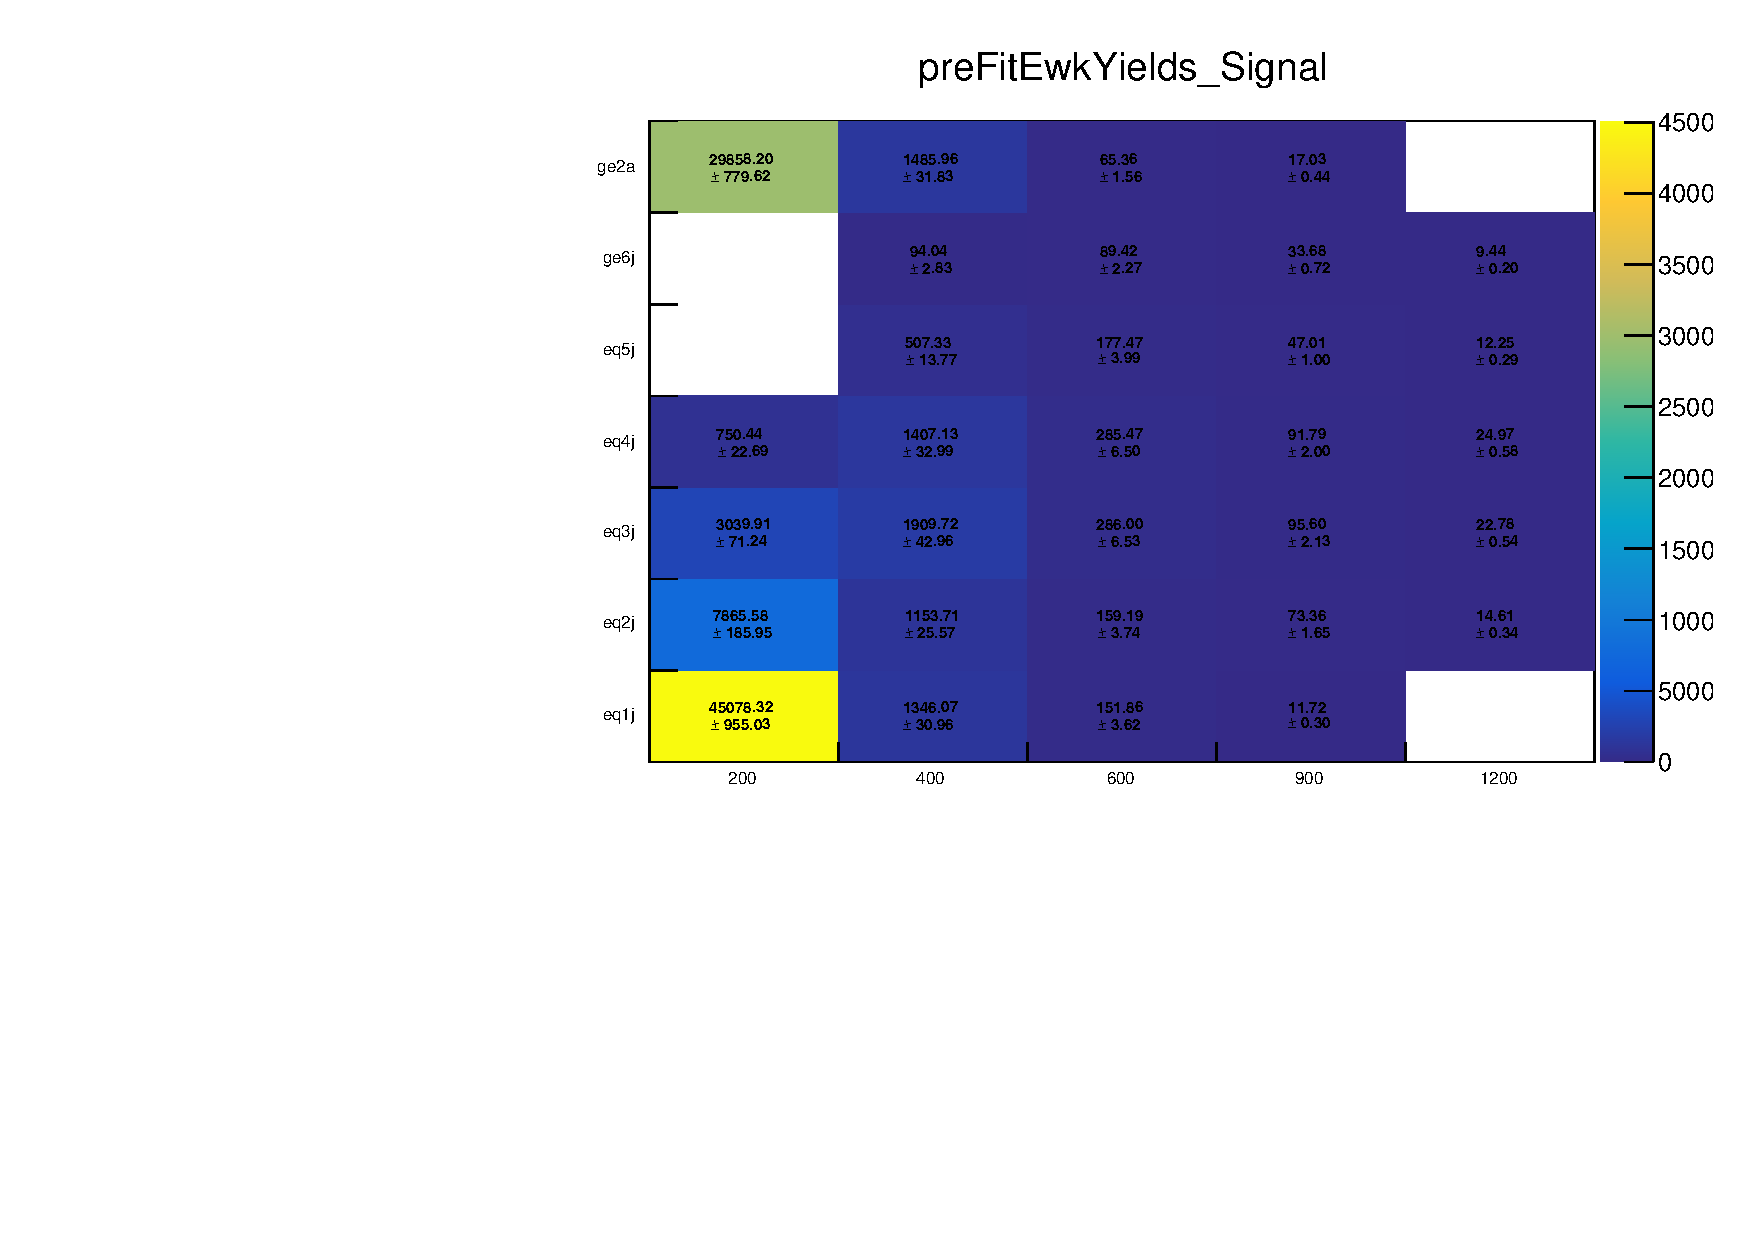
\includegraphics[width=0.6\textwidth]{figures/qcd/qcdANPlots/predictedEwkYields_Signal.pdf}
  } \\
  \subfigure[Ratios of QCD and EWK background estimates.]{
    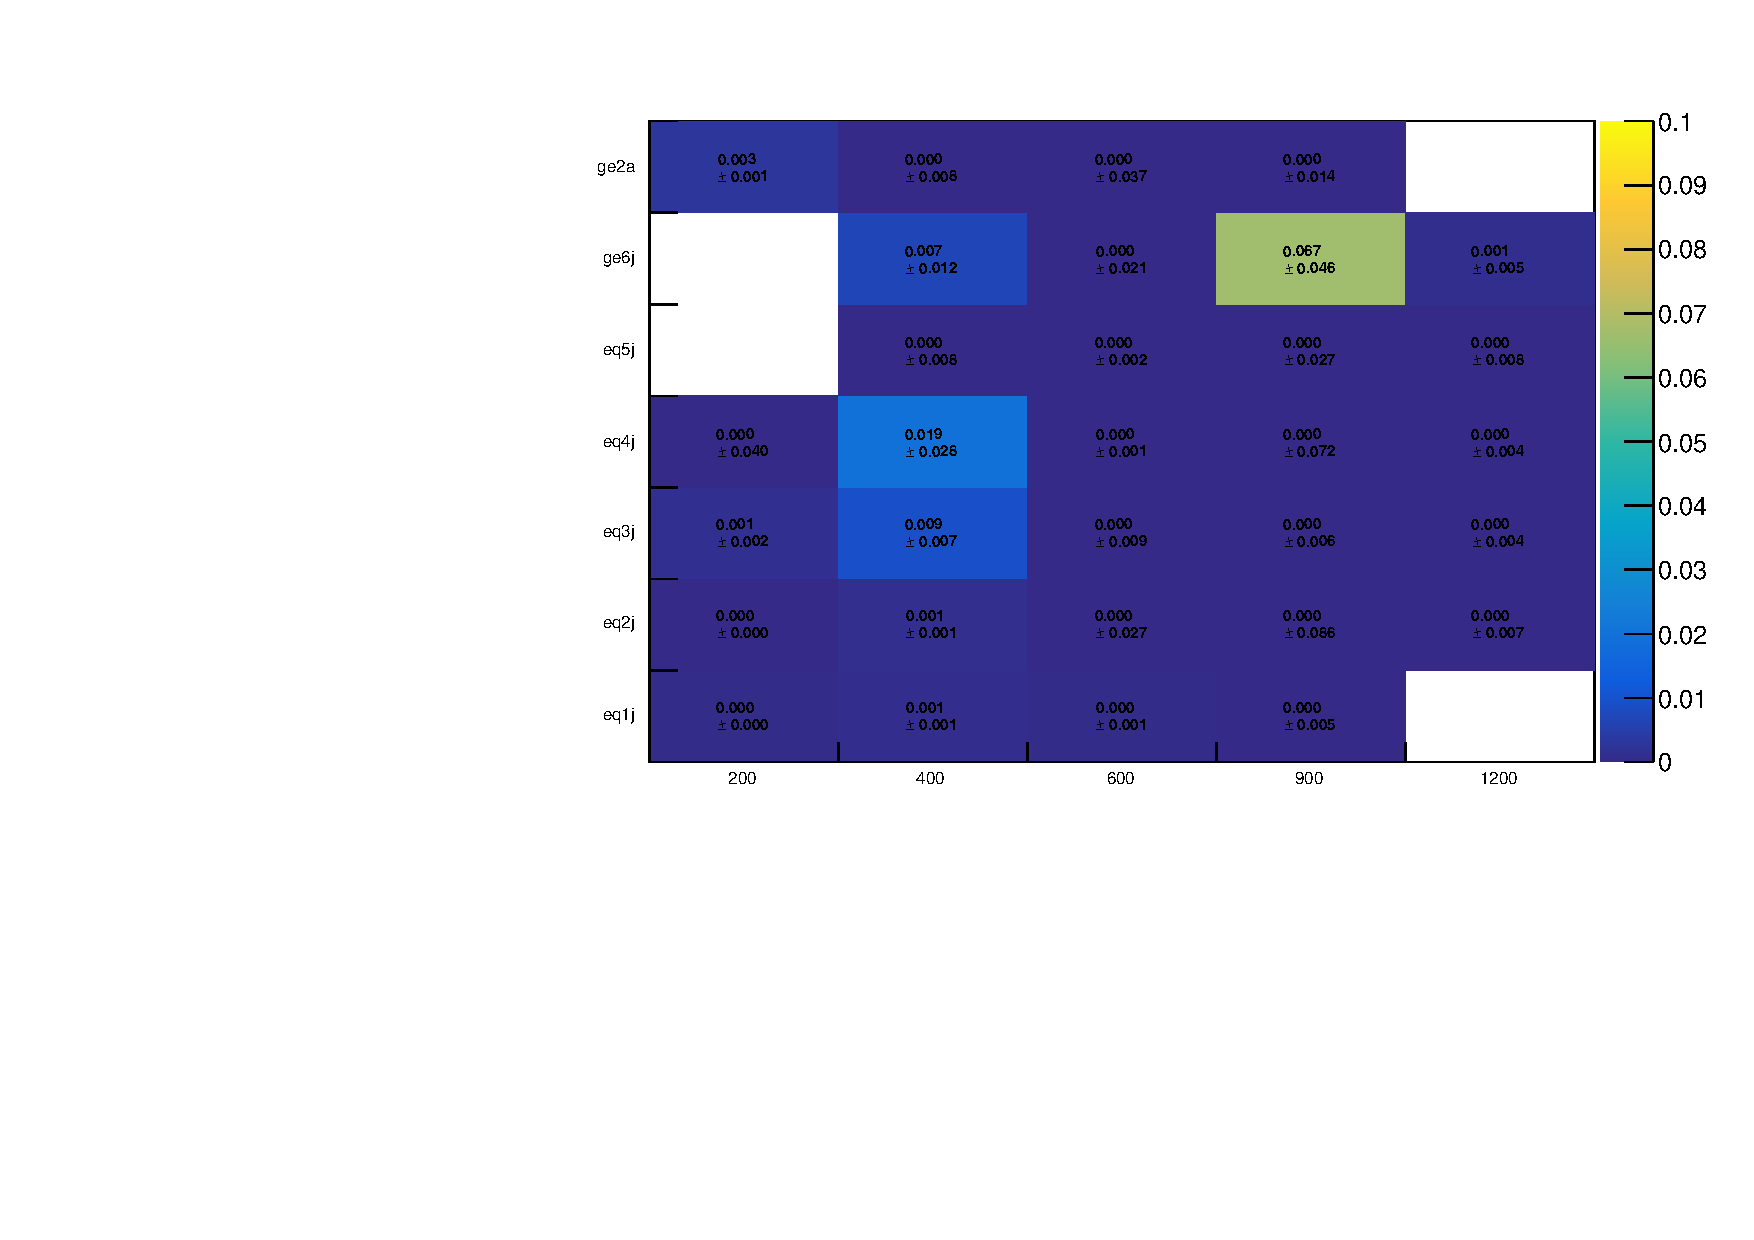
\includegraphics[width=0.6\textwidth]{figures/qcd/qcdANPlots/predictedQcdDivEwk_Signal}
  } 
  \caption{The (a) weighted expected QCD background per (\njet,
    \scalht) bin, (b) the expected EWK background per bin in the
    signal region, and (c) the ratio of the QCD and EWK background
    expectations per bin. }
  \label{fig:qcd_estimate}
\end{figure}

\clearpage
\begin{figure}[!h]
  \centering
  \subfigure[$\mu_{\textrm{QCD}}$(\mhtmet) relative to $\mu_{\textrm{QCD}}$(``double'').]{
    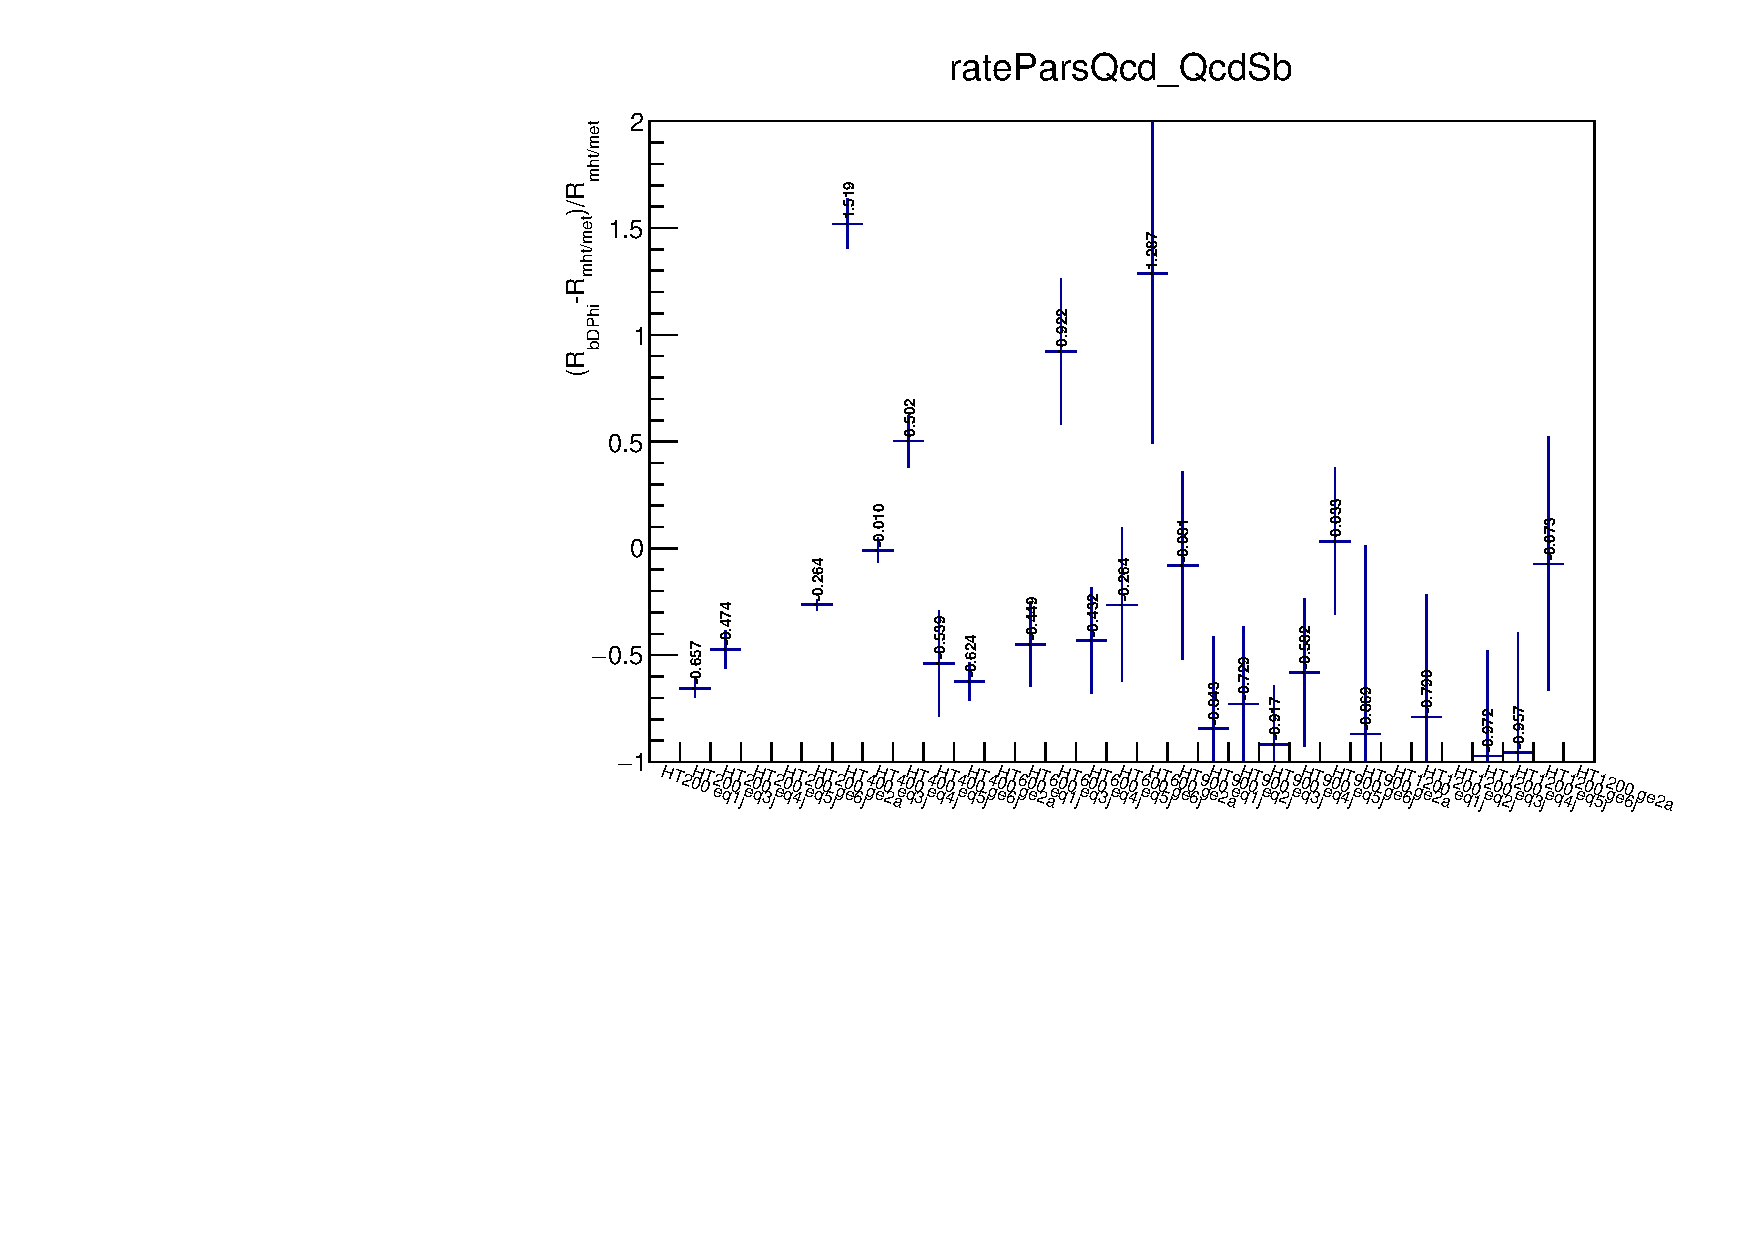
\includegraphics[width=0.8\textwidth]{figures/qcd/newMethod/validation/rateParRatioMhtMetDivBDPhi1d}
  } \\
  \subfigure[$\mu_{\textrm{QCD}}$(\bdphi) relative to $\mu_{\textrm{QCD}}$(``double'').]{
    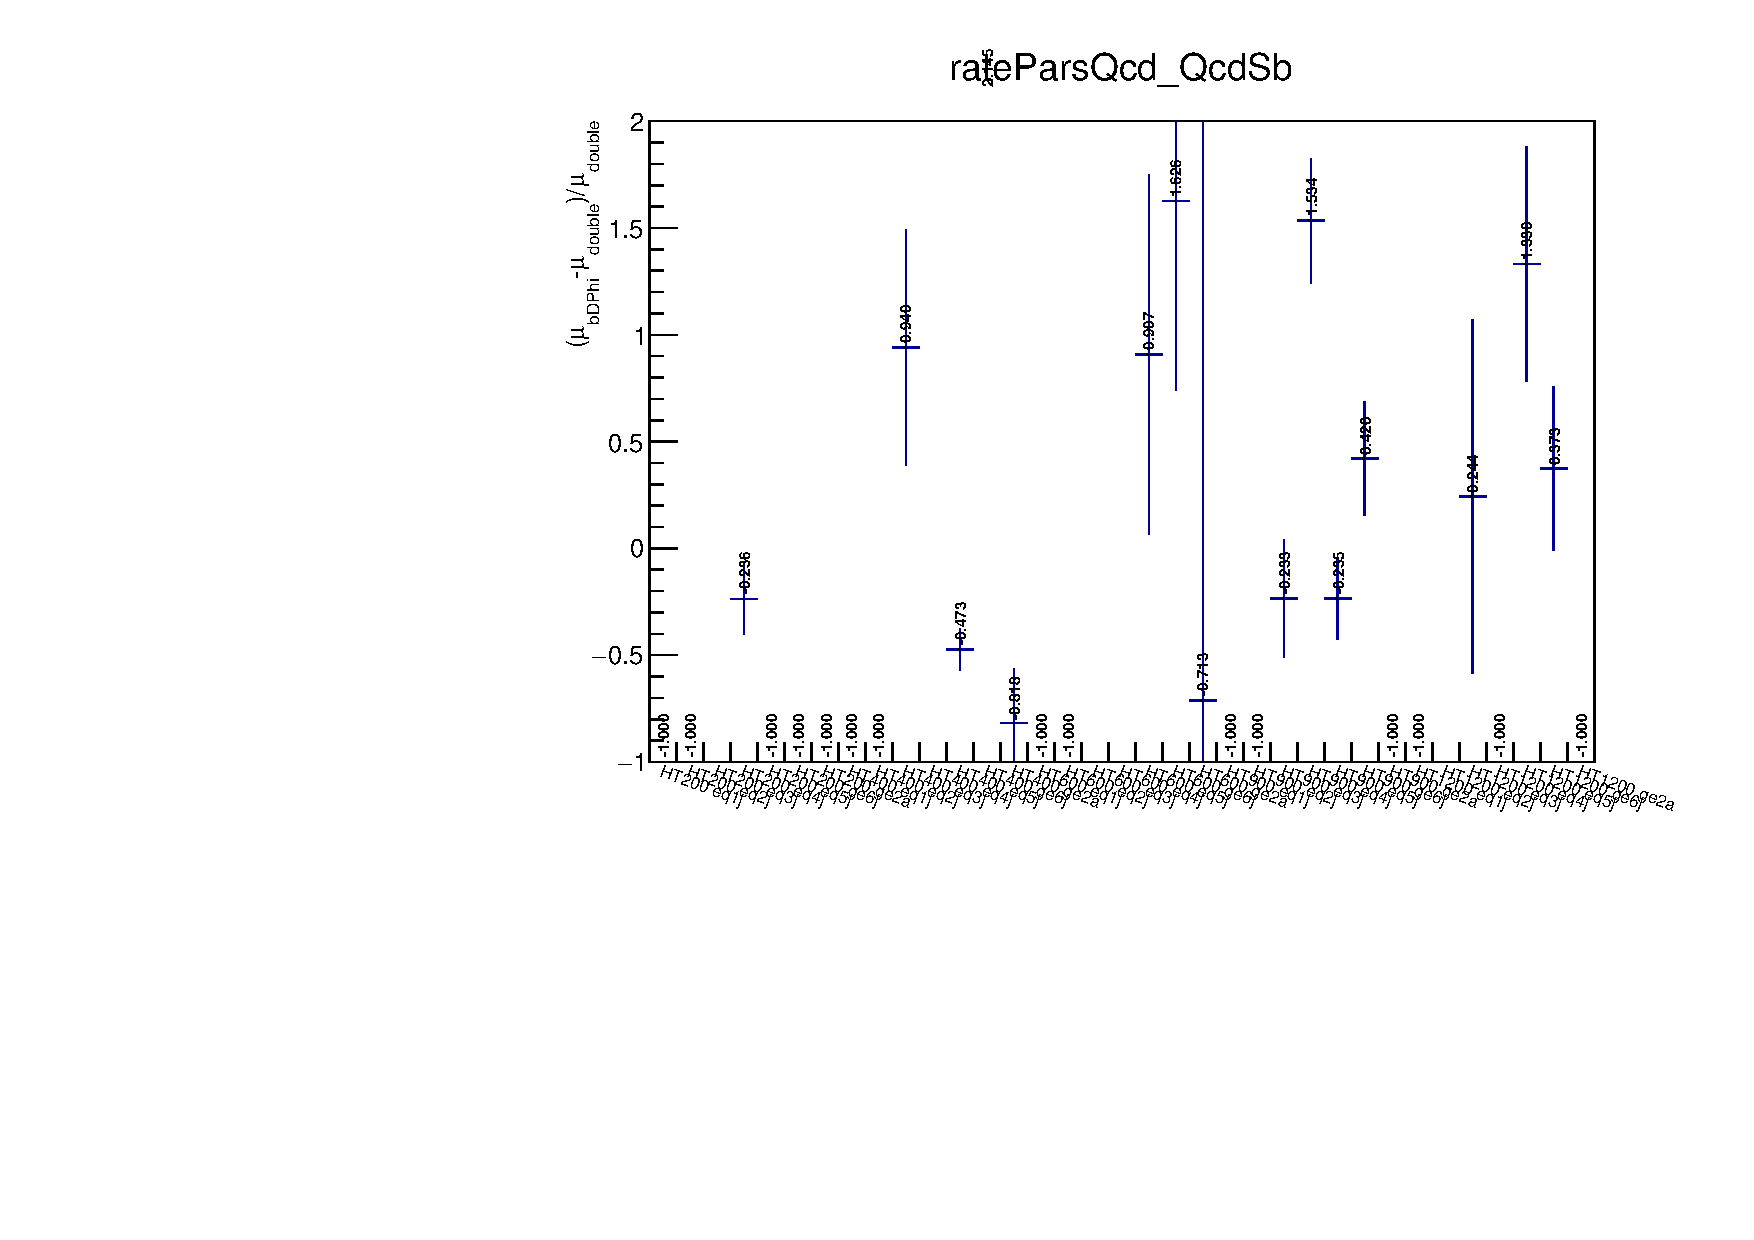
\includegraphics[width=0.8\textwidth]{figures/qcd/newMethod/validation/rateParRatioBDPhiDivDoubleSb1d}
  } 
  \caption{The (fractional) level of agreement between the ML values
    for $\mu_{\textrm{QCD}}$ determined from (a) the \mhtmet and (b)
    the \bdphi sideband regions relative to those obtained from the
    ``double'' sideband region.  }
  \label{fig:qcdVal}
\end{figure}
